\documentclass[11pt]{article}

\usepackage[portuguese]{babel}
\usepackage[T1]{fontenc}
\usepackage[utf8]{inputenc}
\usepackage{amsmath}
\usepackage{graphicx}
\usepackage{subfig}
\usepackage[colorinlistoftodos]{todonotes}
\usepackage{listings}
\usepackage{color} 
\usepackage{float}
\usepackage[font={footnotesize}]{caption}
\usepackage{xcolor,colortbl}
\usepackage{array}
\usepackage{fixltx2e}
\setcounter{secnumdepth}{3}

\numberwithin{equation}{section}

\linespread{1.3}
\usepackage{indentfirst}
\usepackage[top=2.5cm, bottom=2.5cm, right=2.5cm, left=2.5cm]{geometry}



\begin{document}


\begin{titlepage}
	\begin{center}
		
		\hfill \break
		\hfill \break
		
		
\includegraphics[width=0.4\textwidth]{./logo}~\\[1cm]
		
		\textsc{\Large Mestrado Integrado em Engenharia Electrotécnica e de Computadores}\\[1.5cm]
		\textsc{\huge Sistemas Electrónicos de Processamento de Sinal}\\[0.4cm]
		
		{\huge \bfseries Desenvolvimento de um Modulador BPSK com uso de \textit{Costas Loop} \\[1.2cm]}
		
		Grupo n.º 3 \vspace{0.3cm}
		
		\begin{tabular}{l r}
			André Filipe Barroso Cerqueira \hspace{1mm} & n.º 65144 \\
			Guilherme Branco Teixeira \hspace{1mm} & n.º 70214  \\
			João André Catarino Pereira & n.º 73527
		\end{tabular}
		
		\hfill
		\hfill
		
		segunda-feira 15h30 - 18h30, LE1
		
	
		\vfill
		
		{\large Lisboa, 1 de Junho de 2015} 
		
	\end{center}
\end{titlepage}
\pagenumbering{gobble}
\clearpage

	\footnote{As linhas de código apresentadas durante o relatório têm como objectivo demonstrar a maneira de raciocinar na resolução de problemas, não representando uma cópia exata do código usado em laboratório, podendo até, serem consideradas \textit{pseudo-código}}
	
\tableofcontents
\pagebreak

\clearpage
\pagenumbering{arabic}

\section{Introdução}
\todo{mudar introdução}
Este trabalho consiste na primeira parte do projeto de laboratório da cadeira: desenvolvimento de um modem de $Binary$ $Phase$ $Shift$ $Keying$ (BPSK). 

Teve como objectivo a familiarização com o ambiente de desenvolvimento integrado de DSP que consiste nas placas de desenvolvimento DSK TMS320C6416 e DSK TMS320C6713 da $Texas$ $Instruments$ e no software de desenvolvimento $Code Composer Studio v5.5$. Neste projeto foi utilizada a placa DSK TMS320C6713. Foram estudados dois projetos exemplo (sine8\_buf e loop\_intr) e, usando as ferramentas de debug, alteraram-se certos parâmetros de forma a observar os efeitos nos sinais resultantes. Também se consolidaram os conhecimentos adquiridos desenvolvendo dois projetos: um oscilador sinusoidal controlado numericamente e um transmissor BPSK. Os projetos desenvolvidos foram incorporados nos anexos A e B, podendo analisar os mesmos com maior detalhe nos anexos.

\section{Projecto}

\subsection{Projectos de Demonstração}
Foram analisados dois projetos de demonstração com o intuito de familiarizar com os equipamentos e as principais rotinas do projeto.

\subsubsection{sine8\_buf}
\label{sec:sine8}
O objectivo deste projeto é representar a função sinusoidal, multiplicada por um determinado ganho, através de um conjunto de amostras que equivalem a um período da mesma, repetindo nos períodos seguintes esse mesmo conjunto. Este procedimento é realizado através da rotina de interrupção presente no programa. 

Ao analisar o código deste projeto, à primeira vista podemos concluir logo que este usa uma frequência de amostragem de 8 kHz , tem um ganho $G=10$ predefinido e usa 8 amostras para representar a sinusoide. Depois de observar a sinusoide no osciloscópio variou-se o ganho a fim de perceber a sua influência e também o seu limite.
 
Para compreender o limite desta sinusoide é necessário ter em conta que se usa o formato de vírgula fixa Q15 para as suas amostras. Este formato tem como limite o valor $(2^{15}-1) = 32767$. Considerando o valor máximo da sinusoide, se multiplicarmos a mesma por um ganho $G=33$ obtemos um valor superior ao permitido pelo formato Q15 (\textit{overflow}), fazendo com que nesses pontos o valor da sinusoide seja o inverso do que deveria ser, ou seja ocorre \textit{wraparound} na variável da sinusóide (como se poderia esperar dado que se programa em C).
%nao gostou da expressao "caia" para uma tirada da wikipedia}   

\subsubsection{loop\_intr}
\label{sec:loop}
Este projeto fornece-nos um template para os próximos projetos, em termos de comunicação com a placa e rotina de interrupção. Pode-se observar nas últimas linhas de código como se liga os sinais de entrada e saída aos canais da placa.

%interpretar!!                                                                                                                                                                                                                                           
No projeto anterior observou-se os efeitos de \textit{overflow} de uma variável. Neste observam-se os efeitos de aliasing  devido ao sinal de line-in ter a mesma frequência que a frequência de amostragem. A partir dos 4kHz deixamos de ver uma sinusoide com os 3.3V. Não foi feita a experiência de mudar para sinal quadrado e variar a frequência, mas provavelmente não se iria ver um sinal quadrado pois o espectro (infinito) deste teria que ser filtrado pelo anti-aliasing filter. 
\todo{Não me lembro do resultado do sinal quadrado, mas se a sinusóide desapareceu é porque tem filtro anti-aliasing... O que meto aqui?}

\subsection{BPSK Modem}
Este projeto é constituído por duas partes, a primeira é um oscilador controlado numericamente e a segunda é um transmissor BPSK. Devido à existência de um inversor na placa utilizada deu-se, ao longo deste projeto, atenção ao efeito do inversor nos sinais, como se poderá observar nas próximas secções.

\subsubsection{P1. Oscilador controlado numericamente}
\label{NCO}
Usou-se o projeto descrito na secção \ref{sec:loop} como base para a construção de um oscilador controlado numericamente (\textit{NCO}). Um \textit{NCO} é um gerador de sinal digital que cria uma forma de onda discretamente representada no tempo e na amplitude. O \textit{NCO} tem as seguintes características:

\begin{table}[H]
	\centering
	\caption{Características do \textit{NCO} a construir.}
	\label{tab:NCO-car}
\begin{tabular}[c]{|l||c|c|}
	\hline \textbf{Parâmetro} & \textbf{Símbolo} & \textbf{Valor} \\ 
	\hline Frequência de amostragem & $ f_{s} $ & $ 16 kHz $ \\ 
	\hline Frequência mínima & $ f_{min} $ & $ 2 kHz $ \\ 
	\hline Frequência máxima & $ f_{max} $ & $ 6 kHz $ \\ 
	\hline
\end{tabular}
\end{table}

O projeto de construir o \textit{NCO} seguiu os seguintes passos que estão posteriormente explicados:

\begin{enumerate}
	\item Oscilador de Relaxação (Integrador de Rampa). 
	\item Look-up-table (LUT). 
	\item Obtenção de um sinal sinusoidal através da LUT.
	\item Criação de variáveis para controlo da frequência e amplitude do sinal sinusoidal.
	\item Utilização do sinal de entrada para controlar a frequência do sinal.
	\item Teste do oscilador com uma onda sinusoidal à entrada.
	\item Melhoria da qualidade do oscilador com interpolação linear.  
	\item Comparação dos espectros com e sem interpolação.
\end{enumerate}
%\pagebreak

\paragraph{1.Oscilador de Relaxação} \hspace{0pt}

Para construir um Oscilador de Relaxação foi criada uma rotina que, em cada ciclo, incrementa a variável de amplitude do sinal de saída de modo a que este tenha o comportamento de uma rampa. Para que esta tenha precisão máxima e amplitude máxima de 1 V foi usado o formato Q15 para representar o sinal de saída, pois este formato tem amplitude máxima de $2^{15}-1 = 32767 $.\todo{eliminei a frase do múltiplo}

Tendo em conta as frequências da tabela \ref{tab:NCO-car}, podemos chegar aos seguintes valores de incremento com as suas frequências correspondentes.                      
\begin{table}[H]
	\centering
	\caption{Valores a atribuir ao incremento do sinal na saída.}
	\label{tab:incrementos}
	\begin{tabular}[c]{|l||c|}
		\hline \textbf{Frequência de saída($f_0$)} & \textbf{Incremento($\Delta$)}\\ 
		\hline $ 2 kHz \quad (f_{min}) $ & $ 8192 $\\ 
		\hline $ 4 kHz $ & $ 16384 $  \\ 
		\hline $ 6 kHz \quad (f_{max}) $ & $ 24576 $ \\ 
		\hline
	\end{tabular}
\end{table}

Os valores na tabela \ref{tab:incrementos} foram calculados através da seguinte fórmula:
\begin{equation}
 f_{0}= \frac{\Delta}{2A}f_{s} \Leftrightarrow \Delta= 2A\frac{f_{0}}{f_{s}} \hspace{3 mm}, A=32767
\end{equation}
Esta equação trata-se de determinar quantos incrementos se faz de -32767 a 32767 ($2A$), de modo a que ocorra wraparound, sabendo que em cada ciclo da frequência de amostragem $T_s=\frac{1}{f_s}$ se faz um incremento $\Delta$ para se ter um período de rampa $T_0=\frac{1}{f_0}$.
\todo{ja expliquei a expressão}
Foi então possível obter as seguintes rampas com diferentes frequências:
\begin{figure}[H]
	\centering
	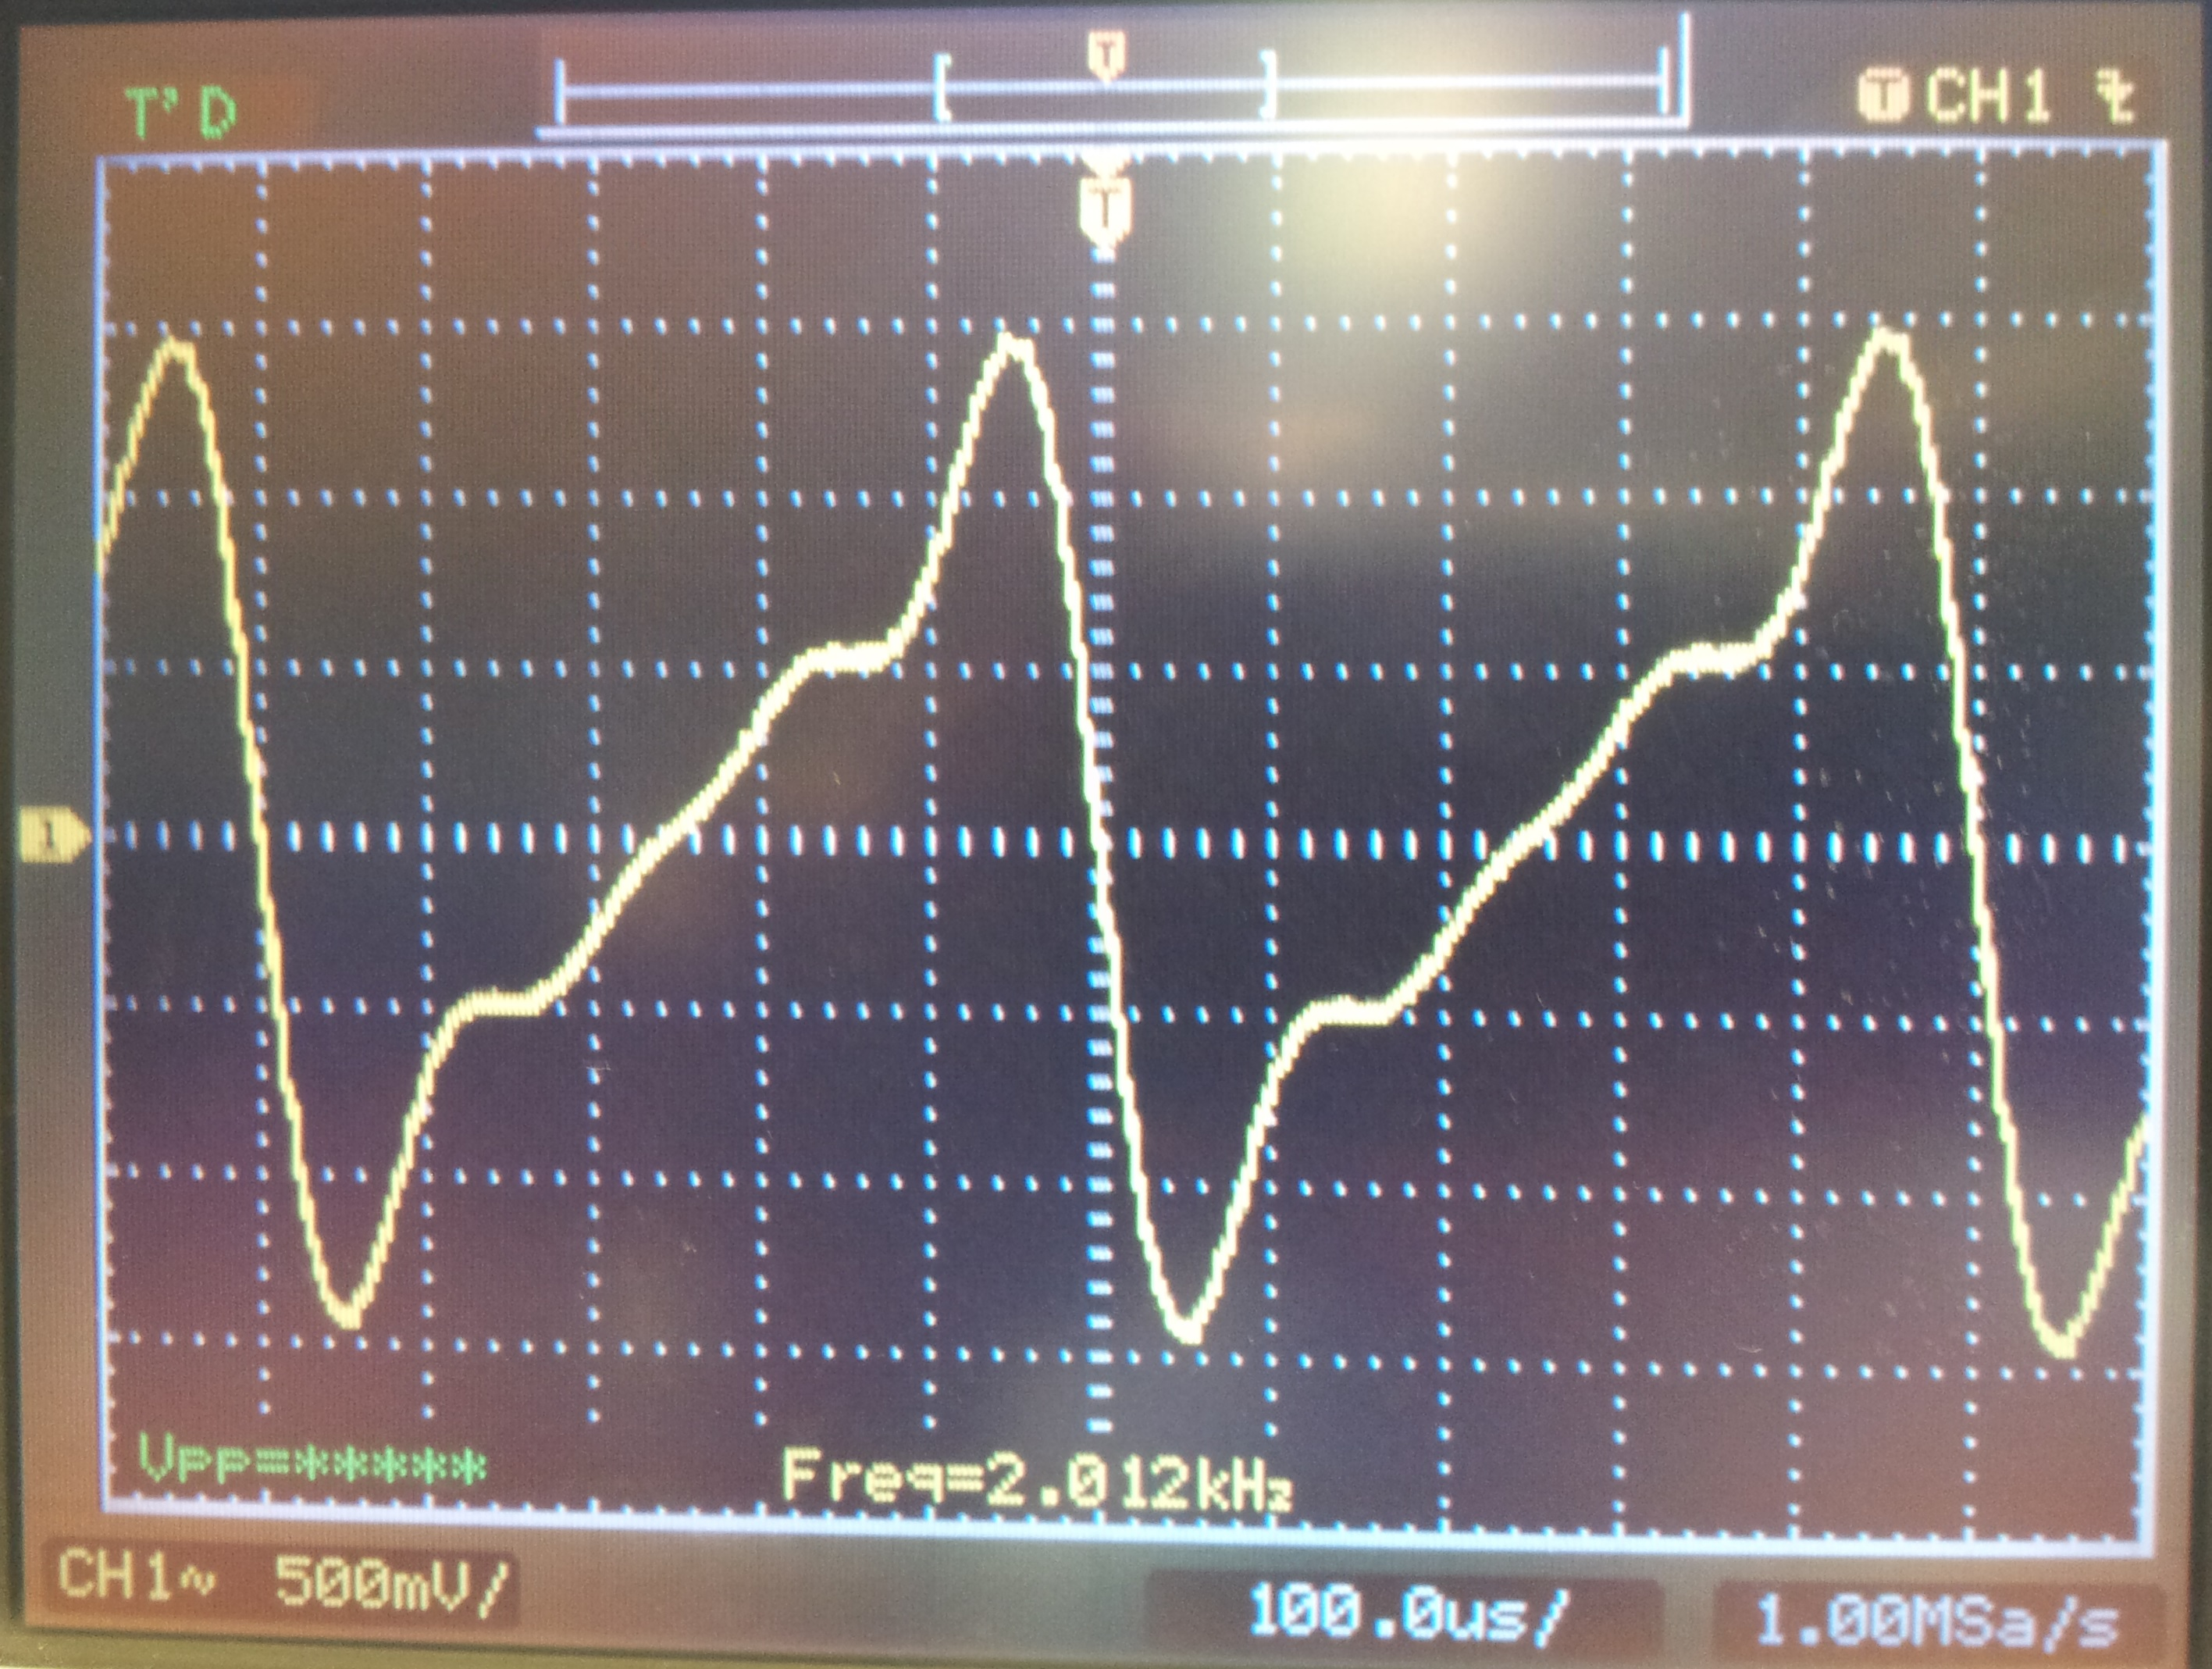
\includegraphics[width=0.5\textwidth]{./P1_2kHz}~\\
	\caption{Rampa com frequência de $ 2 kHz $}
\end{figure}

\begin{figure}[H]
	\centering
	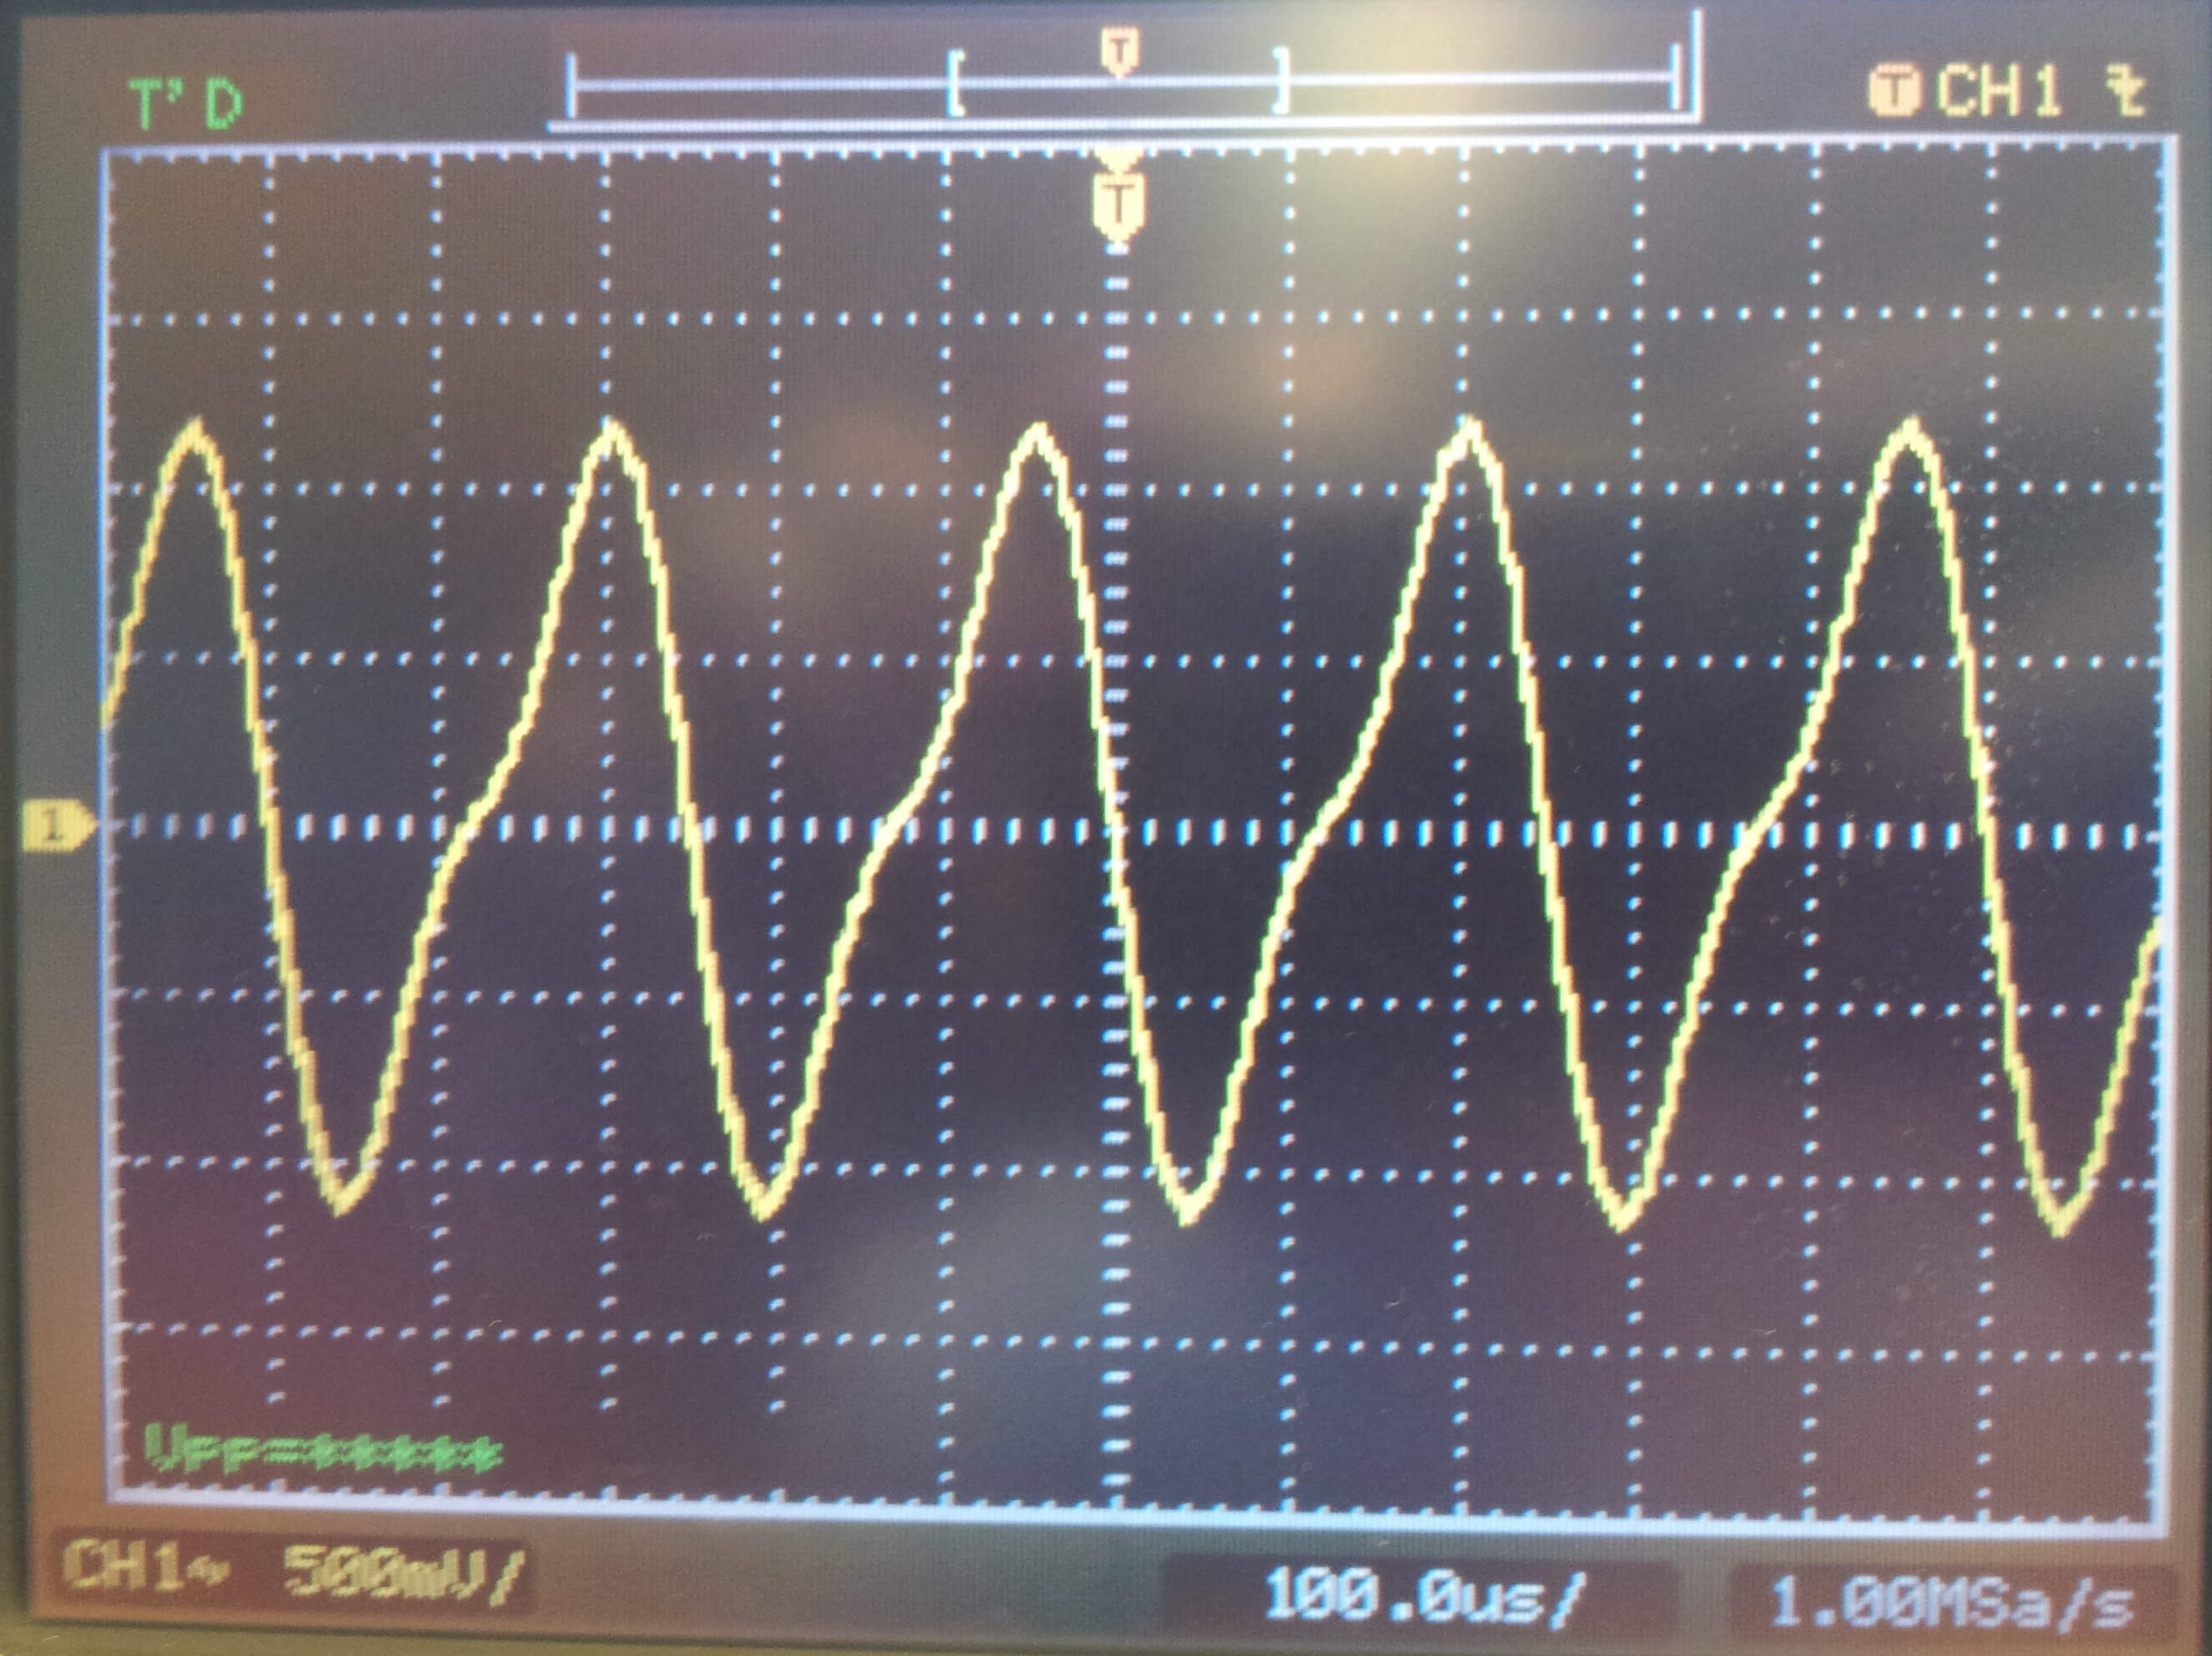
\includegraphics[width=0.5\textwidth]{./P1_4kHz}~\\
	\caption{Rampa com frequência de $ 4 kHz $}
\end{figure}

Ao observar as duas rampas pode-se constatar que para uma frequência mais baixa, ou seja, um incremento menor, a rampa apresenta mais "degraus" e um menor declive. Um incremento menor na rampa significa um maior número de amostras da mesma dentro do intervalo possível, o que reduz o declive da rampa. É de salientar que devido à presença do inversor da placa foi introduzido o simétrico da rampa calculada no canal de modo a observar esta no sentido correto.
\paragraph{2.\textit{Look-up-table}} \hspace{0pt}

Foi criada uma tabela (LUT) com os valores em Q15 de meio ciclo de um seno de modo a que seja possível retirar os seus valores para criar um sinal sinusoidal. Esta tabela tem 32 valores e foi construída com a seguinte equação:

\begin{equation}
round \left(32767*\sin \dfrac{n \pi}{32} \right),  \quad \quad n=0,1,2,...,31
\end{equation}                                                                                                                                                                                                                                             
Para calcular apenas meio ciclo do seno, é necessário ter 32 valores pertencentes ao intervalo $[0,\pi]$ na fase. Assim, é necessário restringir a fase a esse intervalo através da divisão observada na expressão, $\frac{n \pi}{32}$. O produto do seno pelo valor 32767 é a conversão do seno para Q15. 
                                                                     
Não se multiplica por $2 ^{15}=32768$ pois os sinais estão em complemento para dois, o que significa que, para o máximo do seno, esta LUT ultrapassaria o limite do formato, o que causaria \textit{overflow} nessa amostra do sinal resultando num sinal incorreto. \todo{alterei corte para overflow}

Como a tabela LUT inclui apenas meio ciclo de seno, ao criar a sinusoide é necessário negar os valores adquiridos ao criar o segundo meio ciclo do seno.

\paragraph{3.Obtenção de um sinal sinusoidal através da LUT} \hspace{0pt}

Usando como base a rampa criada na secção P1-1 para indexação da LUT criada na secção P1-2, foi possível criar um sinal  sinusoidal.                                                                              

De acordo com o projeto, a rampa é representada num formato Q10, com 1 bit sinal, 5 bits inteiros e 10 bits fraccionários. 
Para a indexação são usados os 5 bits inteiros, ou seja, os 5 mais significativos (excluindo o bit de sinal) do sinal da rampa. Esses 5 bits irão apontar para o valor da tabela de LUT a usar para criar a sinusóide. 
Este processo foi efetuado com o seguinte pedaço de código dentro do ciclo:

\begin{lstlisting}
	rampa=rampa+delta;    //Criar a rampa
	index=rampa>>10;
	index=31 & index;         //Usar apenas 5 bits
	sinusoide=LUT[index];
\end{lstlisting}

Como se pode observar, para isolar os 5 bits inteiros fez-se dez \textit{shifts} para a direita de maneira a ter um sinal apenas com zeros, o bit sinal e esses 5 bits encostados à direita. A seguir aplicou-se uma máscara constituída por uma AND com 31 bits, de maneira a retirar o bit sinal e finalmente isolar num sinal o índice pretendido da LUT. Com o índice é uma questão de aceder à tabela e obter \textit{y1}, neste caso representado pelo sinal \textit{sinusoide} (Figura \ref{fig:sen2k}).

\begin{figure}[H]
	\centering
	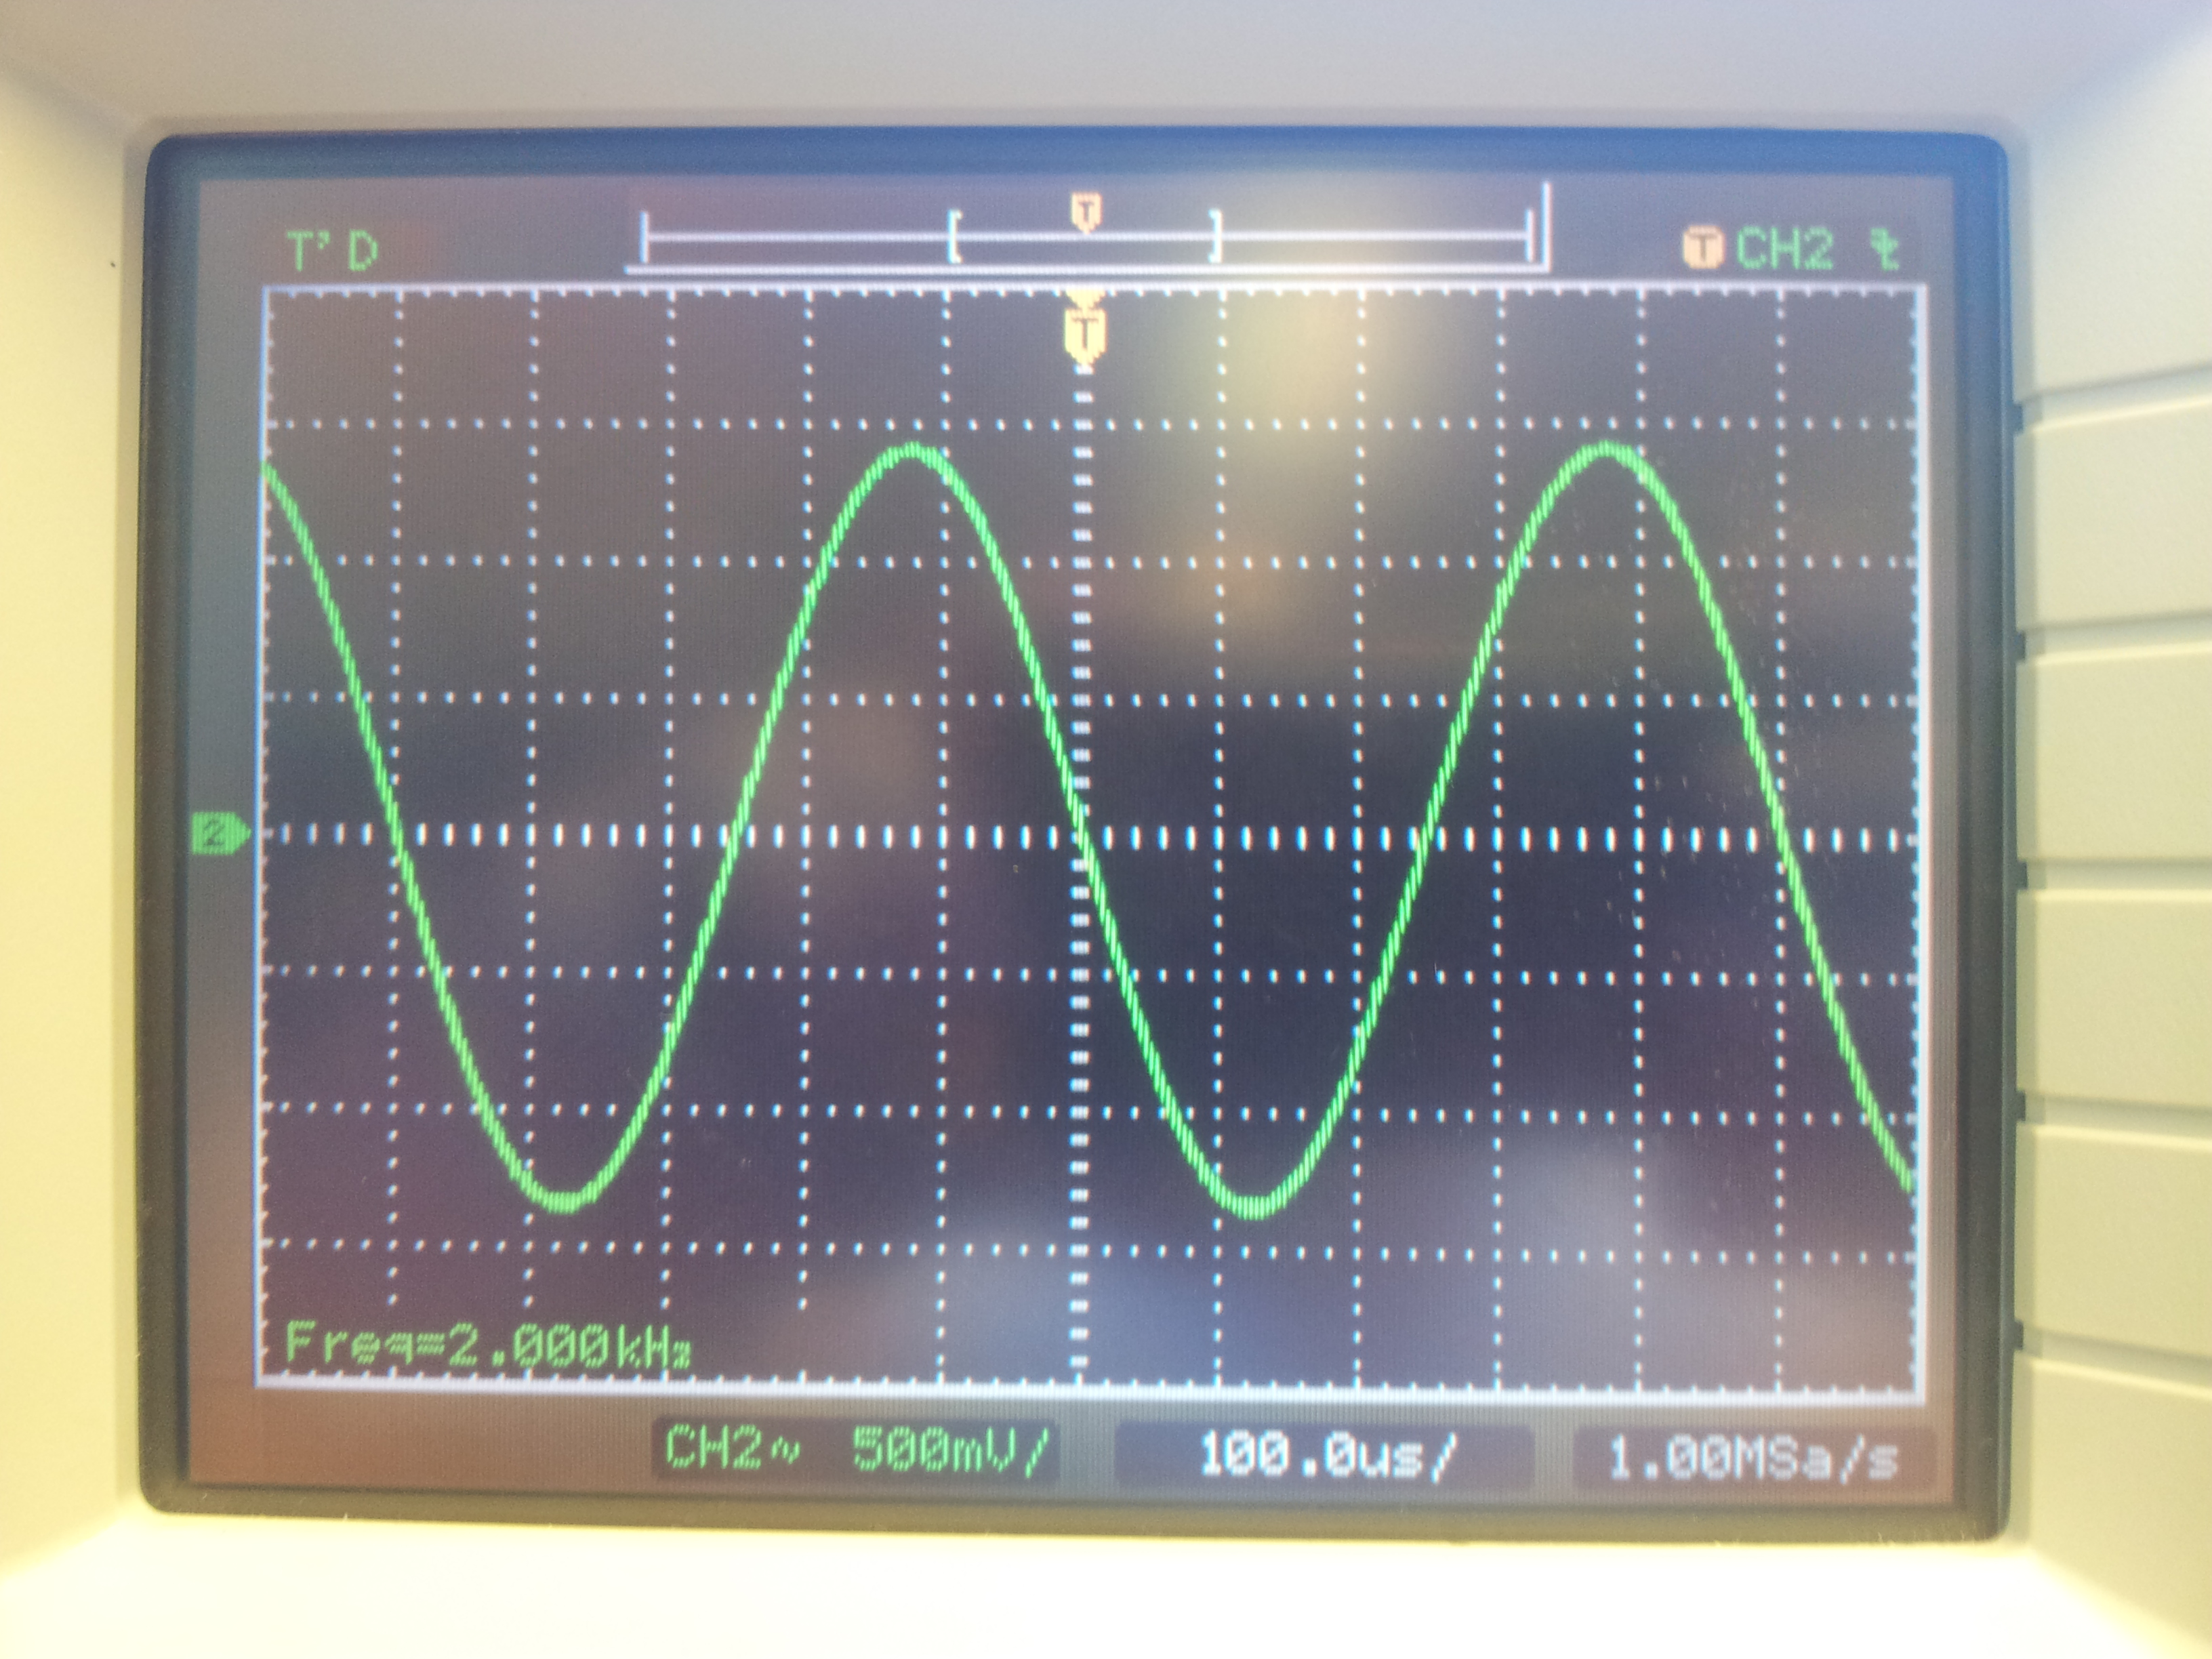
\includegraphics[width=0.5\textwidth]{./P1_1seno}~\\
	\caption{Sinal sinusoidal criado de $ 2 kHz $.}
	\label{fig:sen2k}
\end{figure}

Como se pode observar na figura foi possível criar um sinal aproximadamente sinusoidal através de uma LUT indexada por uma rampa. Nesta figura não é possível notar mas quando se aproxima mais o sinal no osciloscópio verifica-se pequenos degraus ao longo do sinal, que simbolizam a aproximação obtida através das amostras.

\paragraph{4.Criação de variáveis para controlo da frequência e amplitude do sinal sinusoidal} \hspace{0pt}

Foram criadas duas variáveis para que fosse possível controlar a frequência e a amplitude do sinal à saída, \textit{delta} e \textit{ampl}, respectivamente.

A primeira variável foi já antes referida, nas secções P1-1 e P1-3. Esta variável, caso alterada iria alterar a frequência da rampa, e por consequência, a frequência do sinal de saída. Como se pode observar na tabela \ref{tab:incrementos}, esta variável terá como limite máximo o valor $ 24576 $ e como limite mínimo $ 8192 $ devido às frequências mínima e máxima. Podemos também concluir que quanto maior for esta variável, maior a frequência do sinal de saída e também se o seu valor diminuir, a frequência de saída irá diminuir.

A segunda variável (\textit{ampl}) foi criada com o propósito de modelar a amplitude do sinal de saída. Esta causou mudanças mais significativas no código, tal como se pode verificar:

\begin{lstlisting}
	rampa=rampa+delta;
	index=rampa>>10;
	index=31 & index;        
	aux=ampl*LUT[index];
	aux=aux<<1;            //Retirar bit de sinal extra
	sinusoide=-aux>>16;    //Colocar o sinal com 16 bits em Q15
\end{lstlisting}

Esta variável tem como valor máximo $ 32767 $, pois os valores afixados na tabela LUT já apresentam um valor com a amplitude máxima de Q15 de maneira a não ter problemas com o formato de representação nem com a amplitude do sinal transmitido à placa.
Como se pode ver no código a variável \textit{ampl} multiplica diretamente pela LUT. 
\vspace{2 mm}

Quando se multiplica dois sinais, o sinal resultante fica com um bit sinal replicado que é eliminado através de um \textit{shift} esquerdo. Mas depois ainda é necessário ir buscar os 16 bits mais significativos através de 16 \textit{shifts} para a direita pois pretende-se um sinal com 16 bits em Q15. 

Na equação seguinte pode-se observar como obter o formato resultante num produto:
\begin{equation}
Q_{m} * Q_{k}=Q_{m+k-n+1}
\end{equation}
Neste caso como se multiplica dois sinais Q15 e \textit{n}$=$16 bits representa-se o resultado com formato Q15 como foi dito anteriormente.
Com a criação destas variáveis passou-se a ter um oscilador numericamente controlado.

\paragraph{5.Utilização do sinal de entrada para controlar a frequência do sinal} \hspace{0pt}

Para que a frequência do sinal de saída seja modulada através da amplitude do sinal de entrada, é necessário criar uma relação linear entre o sinal de entrada \textit{inbuf} e o incremento da rampa \textit{delta}, pois este é que define a frequência do sinal sinusoidal com a rampa. Como tal a relação entre o \textit{inbuf} e o \textit{delta} é ilustrada pela seguinte equação:
\begin{equation}
	\Delta=\Delta_0+(K*inbuf)	\hspace{6 mm}\Delta_0=16384, K=\frac{1}{4}
	\label{delta}
\end{equation}
Tendo em conta a tabela \ref{tab:incrementos}, delta varia entre 8192 e 24576 com $\Delta_0$ correspondente à frequência central, 4 kHz. Para restringir delta a esse intervalo foi necessário introduzir $K=\dfrac{1}{4}$. Assim, obtém-se uma relação proporcionalmente direta entre delta e o sinal de entrada, o que significa que se aumentar ou diminuir a amplitude do sinal de entrada também aumenta ou diminui o delta.

Pode-se observar a implementação da equação explicada anteriormente, no código seguinte:

\begin{lstlisting}
	delta=16384-(inbuf>>2); 
	rampa=rampa+delta;		//rampa
\end{lstlisting}
O duplo \textit{shift} para a direita é equivalente a dividir por 4 e mais eficiente pois, uma vez que o DSP não possui divisor, evita uma passagem do programa pela ALU, também representando o efeito de K.
Embora na equação (4) se some o valor do \textit{inbuf}, no programa tem que se ter em conta o efeito do inversor na placa e por isso efectua-se uma subtração.

\paragraph{6.Teste do oscilador com uma onda sinusoidal à entrada} \label{para:P1-6} \hspace{0pt}

Para testar o funcionamento do NCO, pôs-se na entrada do DSP um sinal sinusoidal com frequência igual a 2 Hz, como sinal modulante, em vez da onda quadrada pedida no enunciado pois seria mais fácil observar a variação de frequência do sinal de saída se a variação de amplitude do sinal de entrada fosse gradual em vez de ser constante com descontinuidades. 
\vspace{1 mm}

Esperou-se que, no máximo e mínimo de amplitude da sinusoide de entrada, a onda modulada tivesse máxima e mínima frequência respetivamente, e que uma variação na amplitude do sinal modulante provocasse um efeito linear na frequência do sinal modulado. Tal observou-se no osciloscópio, contudo não é possível representar numa figura para referência uma vez que seria necessário uma gravação de vídeo do processo para poder observar a variação pretendida. Para isso ser possível era necessário usar a tal onda quadrada como sinal de entrada.

\paragraph{7.Melhoria da qualidade do oscilador com interpolação linear} \hspace{0pt}

Com o objectivo de melhorar a qualidade do sinal criado vai ser usado o método de interpolação linear descrito na seguinte equação:

\begin{equation}
y=y_{1}+(y_{2}-y_{1})*\Delta_{x}
\end{equation}                       

Sendo que $ \Delta_{x} $ refere-se aos 10 bits menos significativos ignorados na altura em que se retirou da rampa o índice da LUT. O processo de recolher o valor de $ \Delta_{x} $ e do cálculo da interpolação estão descritos nas seguintes linhas de código:
\todo{explicar aritmética do código!!}
\begin{lstlisting}
	rampa=rampa+delta;
	deltaX=1023 & rampa;   //Retirar os 10 bits menos significativos
	deltaX=deltaX<<5;      //Converter deltax em Q15

	(...)
	Y1=-((amplitude*LUT[index])<<1)>>16;	// Y1=LUT(i) convertido para Q15
	Y2=-((amplitude*LUT[(index+1) & 31])<<1)>>16;	// Y2=LUT(i+1) convertido para Q15
	aux=(Y2-Y1)*deltaX;		
	aux=aux<<1;				//Retirar bit de sinal extra
	Y=Y1+(aux>>16);			//interpolacao	
\end{lstlisting}

Como se pode observar nas linhas de código, a interpolação é realizada com dois valores que são retirados da tabela LUT, usando como índice $\textit{index}$ \hspace{0,1 mm} e $(\textit{index}+1)$ respectivamente. Neste método com interpolação estaremos a usar 10 bits, que no método anterior (sem interpolação) foram descartados fazendo um sacrifício na precisão,  estes bits constituem a variável $ \Delta_{x} $ que será usada na equação da interpolação.
                                            
Para isolar a mesma foi usada uma máscara primeiro para retirar os 10 bits que interessam e depois efetuaram-se 5 \textit{shifts} para a esquerda de modo a converter para Q15.

Ambos os sinais (com e sem interpolação) podem ser observados na Figura \ref{fig:interp}, embora a sua comparação não possa ser efetuada por mera observação. Para estes sinais utilizou-se $\Delta_0=20479$ correspondente a $f_0=5kHz$.
\todo{frequência e delta posto}               
\begin{figure}[H]
	\centering                                          
	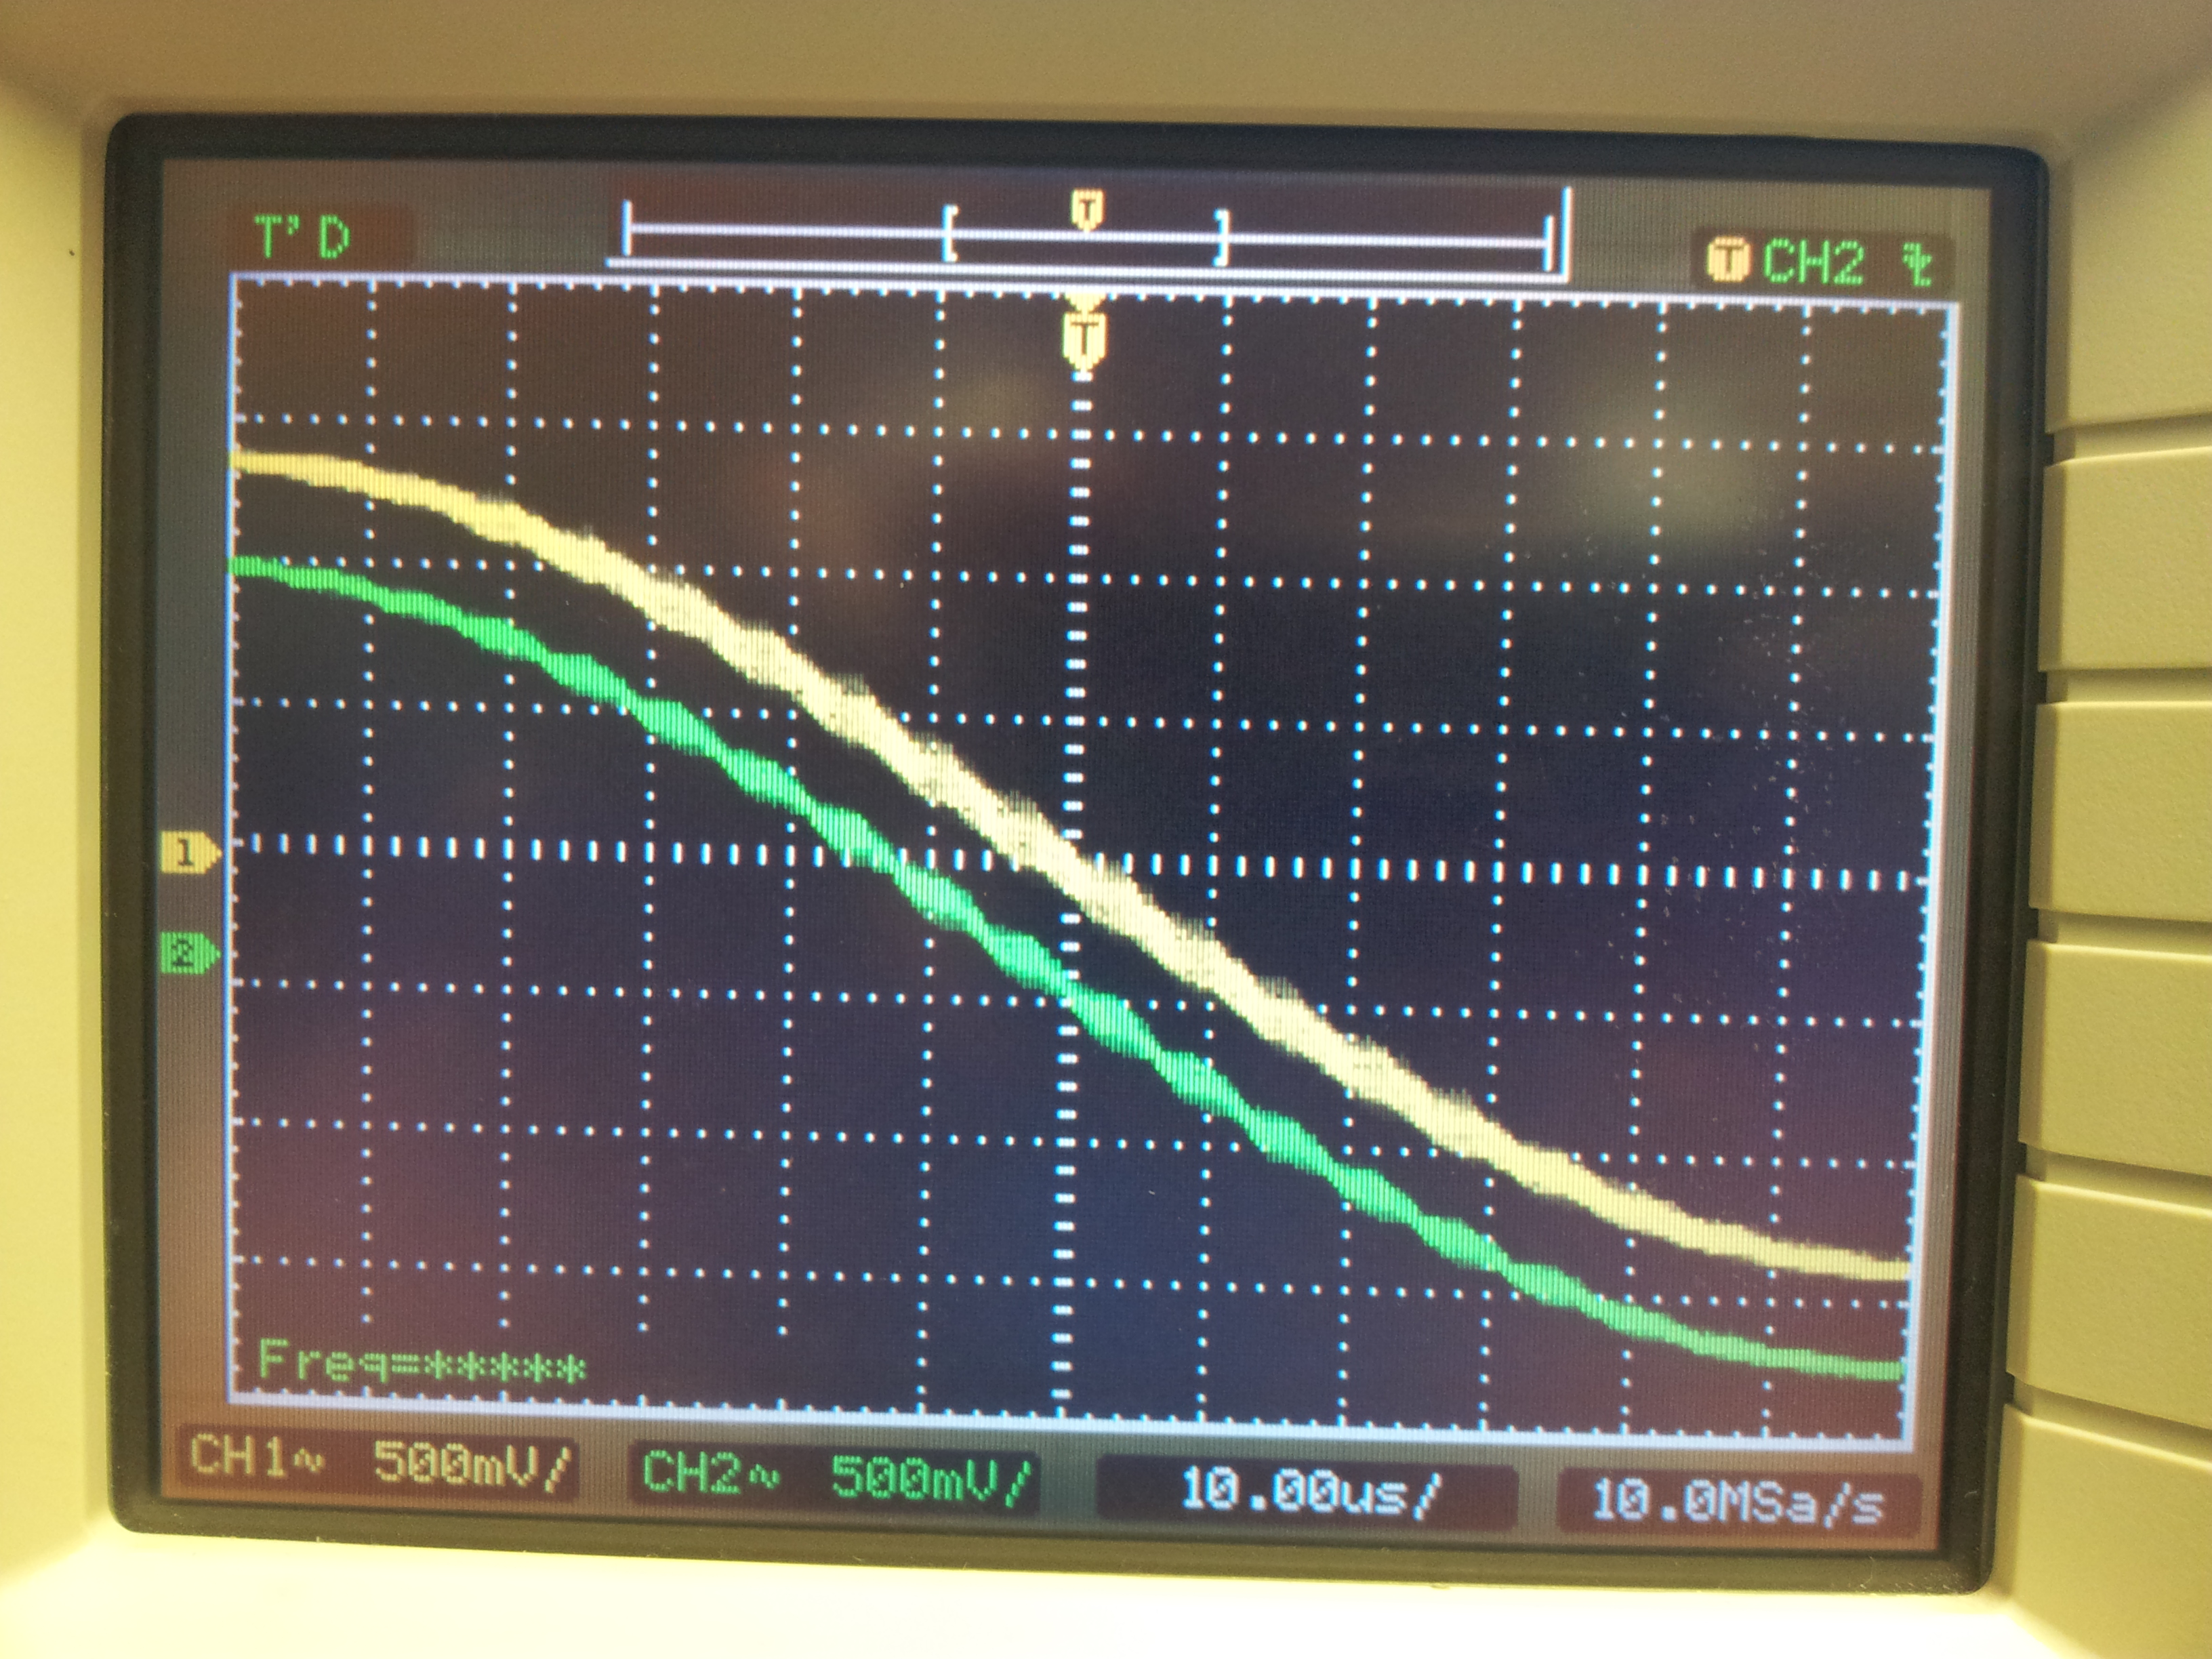
\includegraphics[width=0.5\textwidth]{./P1_interp}~\\
	\caption{Sinal sinusoide com interpolação(amarelo) e sem interpolação(verde).}
	\label{fig:interp}
\end{figure} \todo{pus os canais}
Nesta figura é possível observar os "degraus" mencionados anteriormente, tanto na onda interpolada como na onda não interpolada.

\paragraph{8.Comparação dos espectros com e sem interpolação} \hspace{0pt}

\todo{salientar q se fez pra um delta diferente de 16384}
Não sendo possível estabelecer uma diferença entre os sinais com interpolação e sem interpolação foi necessário recorrer à observação dos espectros deles mesmos (Figuras \ref{fig:espect_s_interp} e \ref{fig:espect_c_interp}).
\begin{figure}[H]
	\centering
	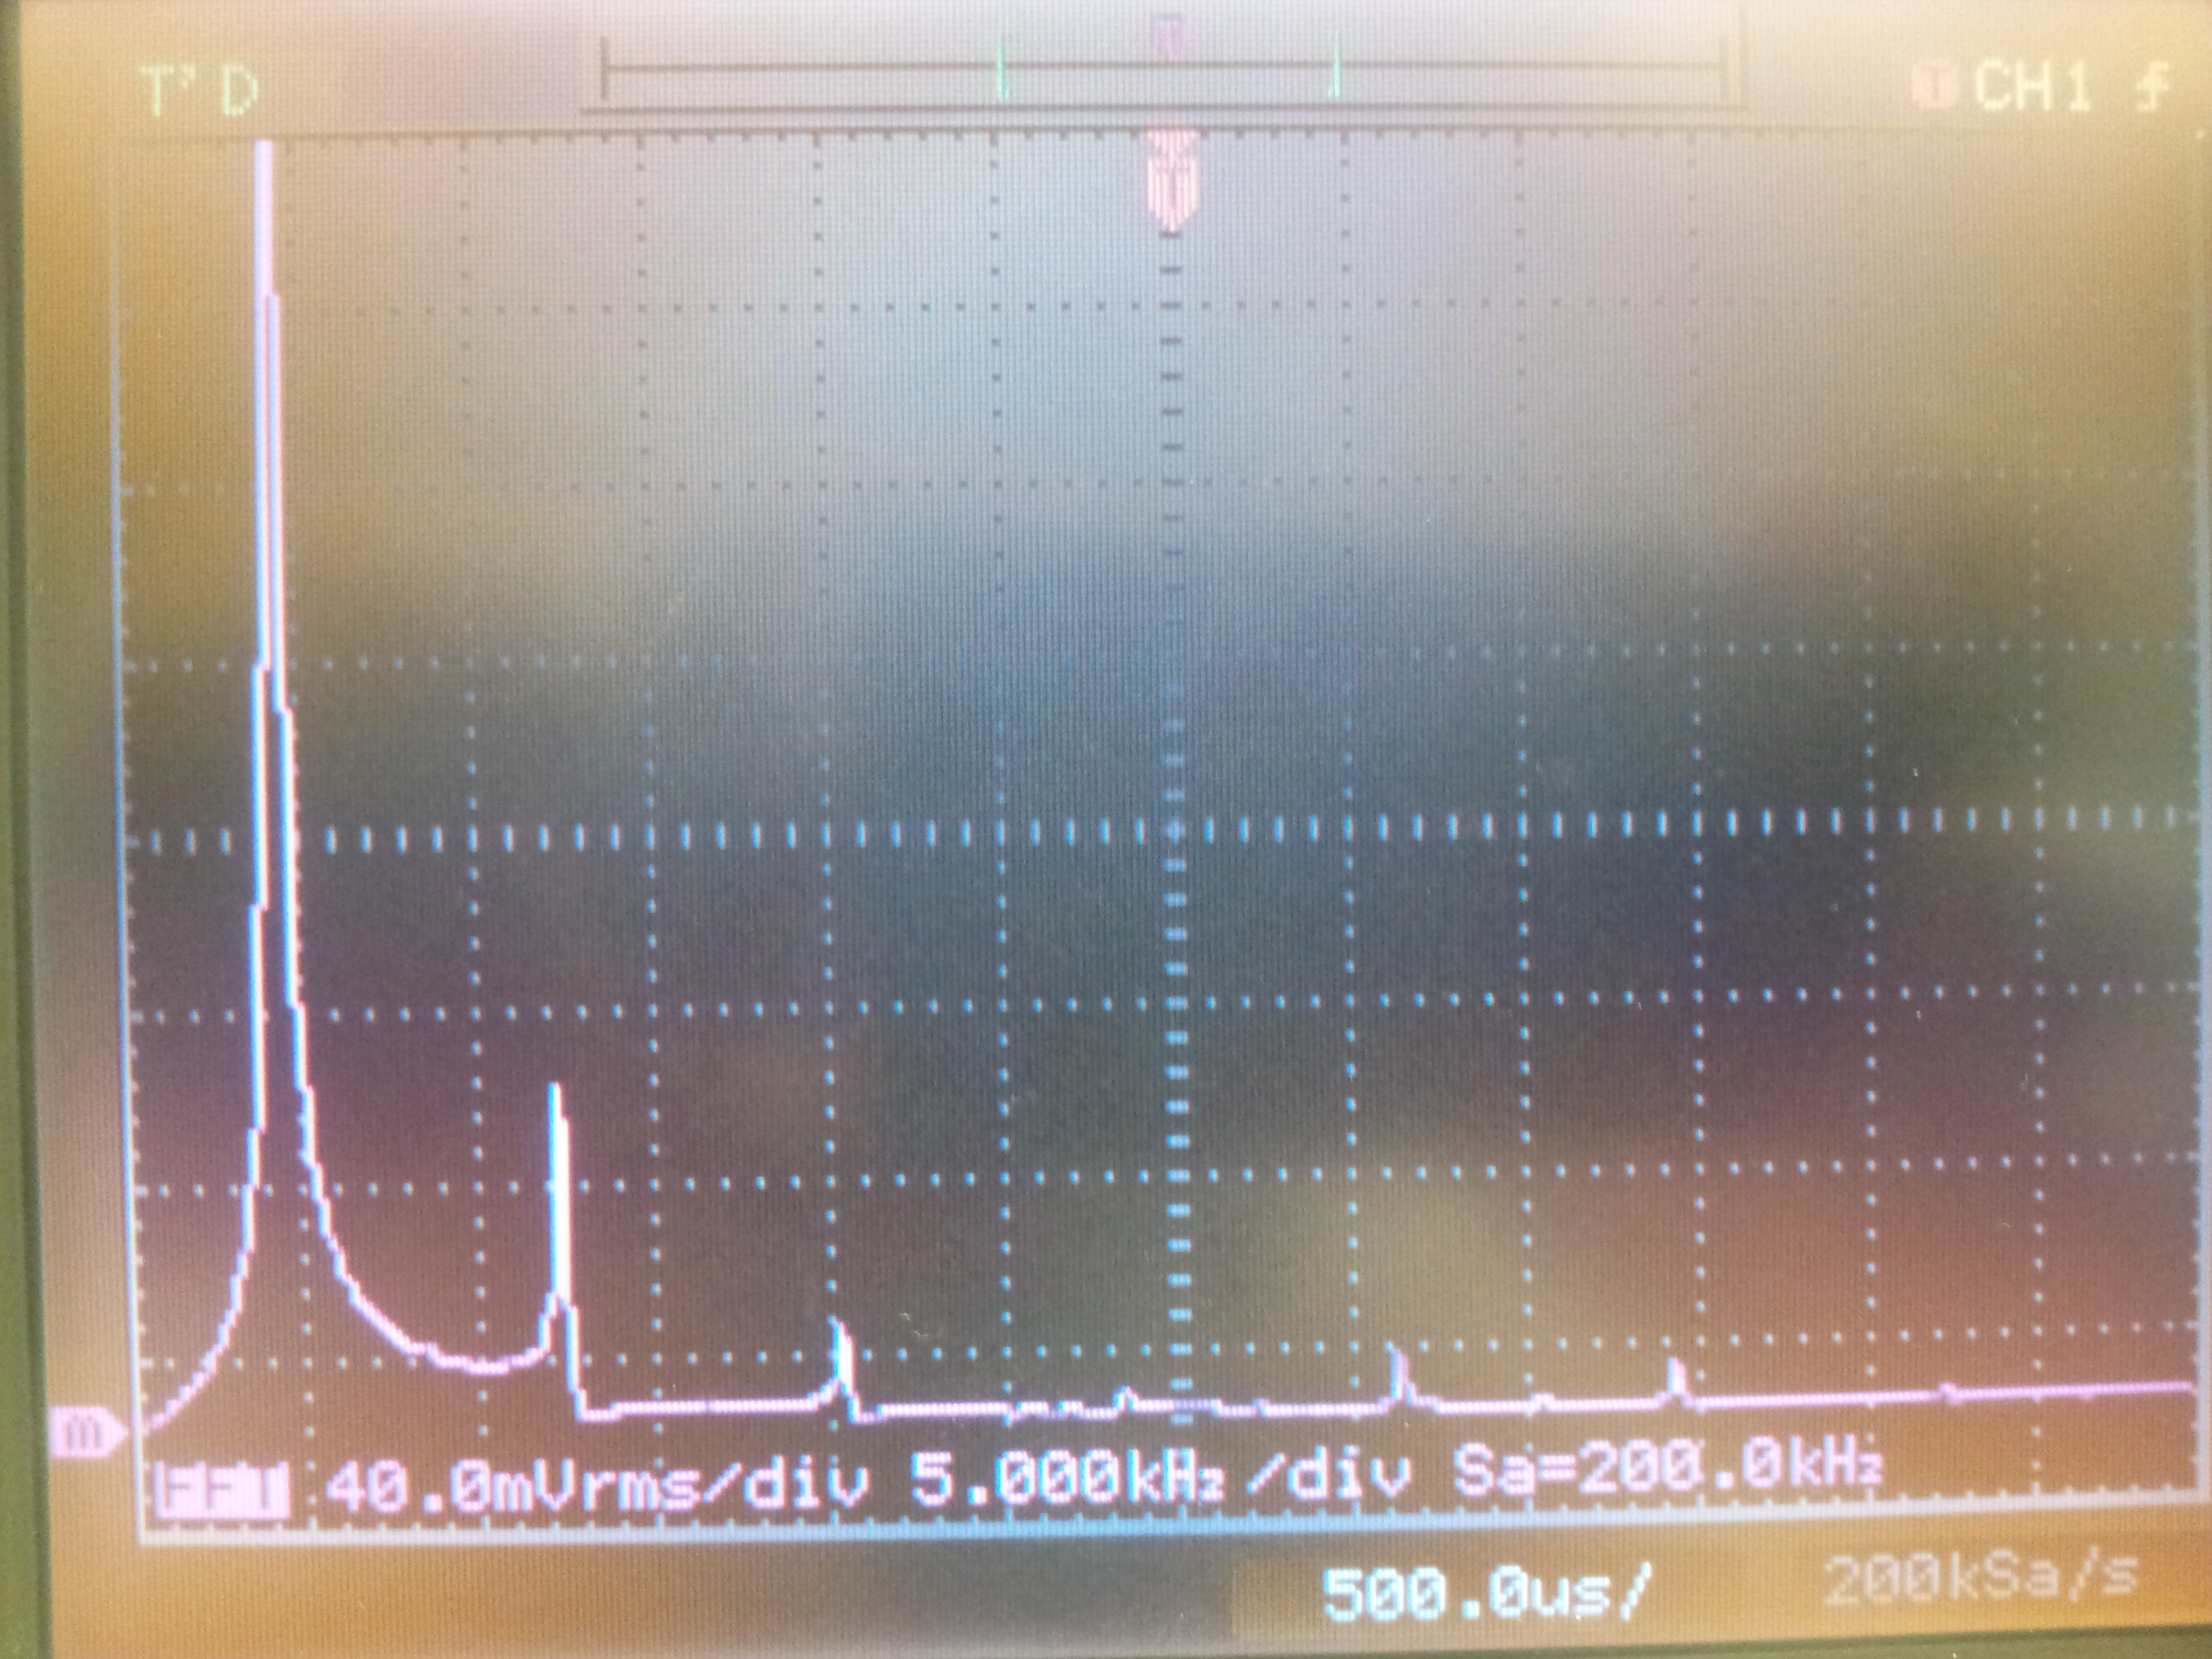
\includegraphics[width=0.5\textwidth]{./P1-8_espect_s_interp}~\\
	\caption{Espectro do sinal sinusoide sem interpolação.}
	\label{fig:espect_s_interp}
\end{figure}

\begin{figure}[H]
	\centering
	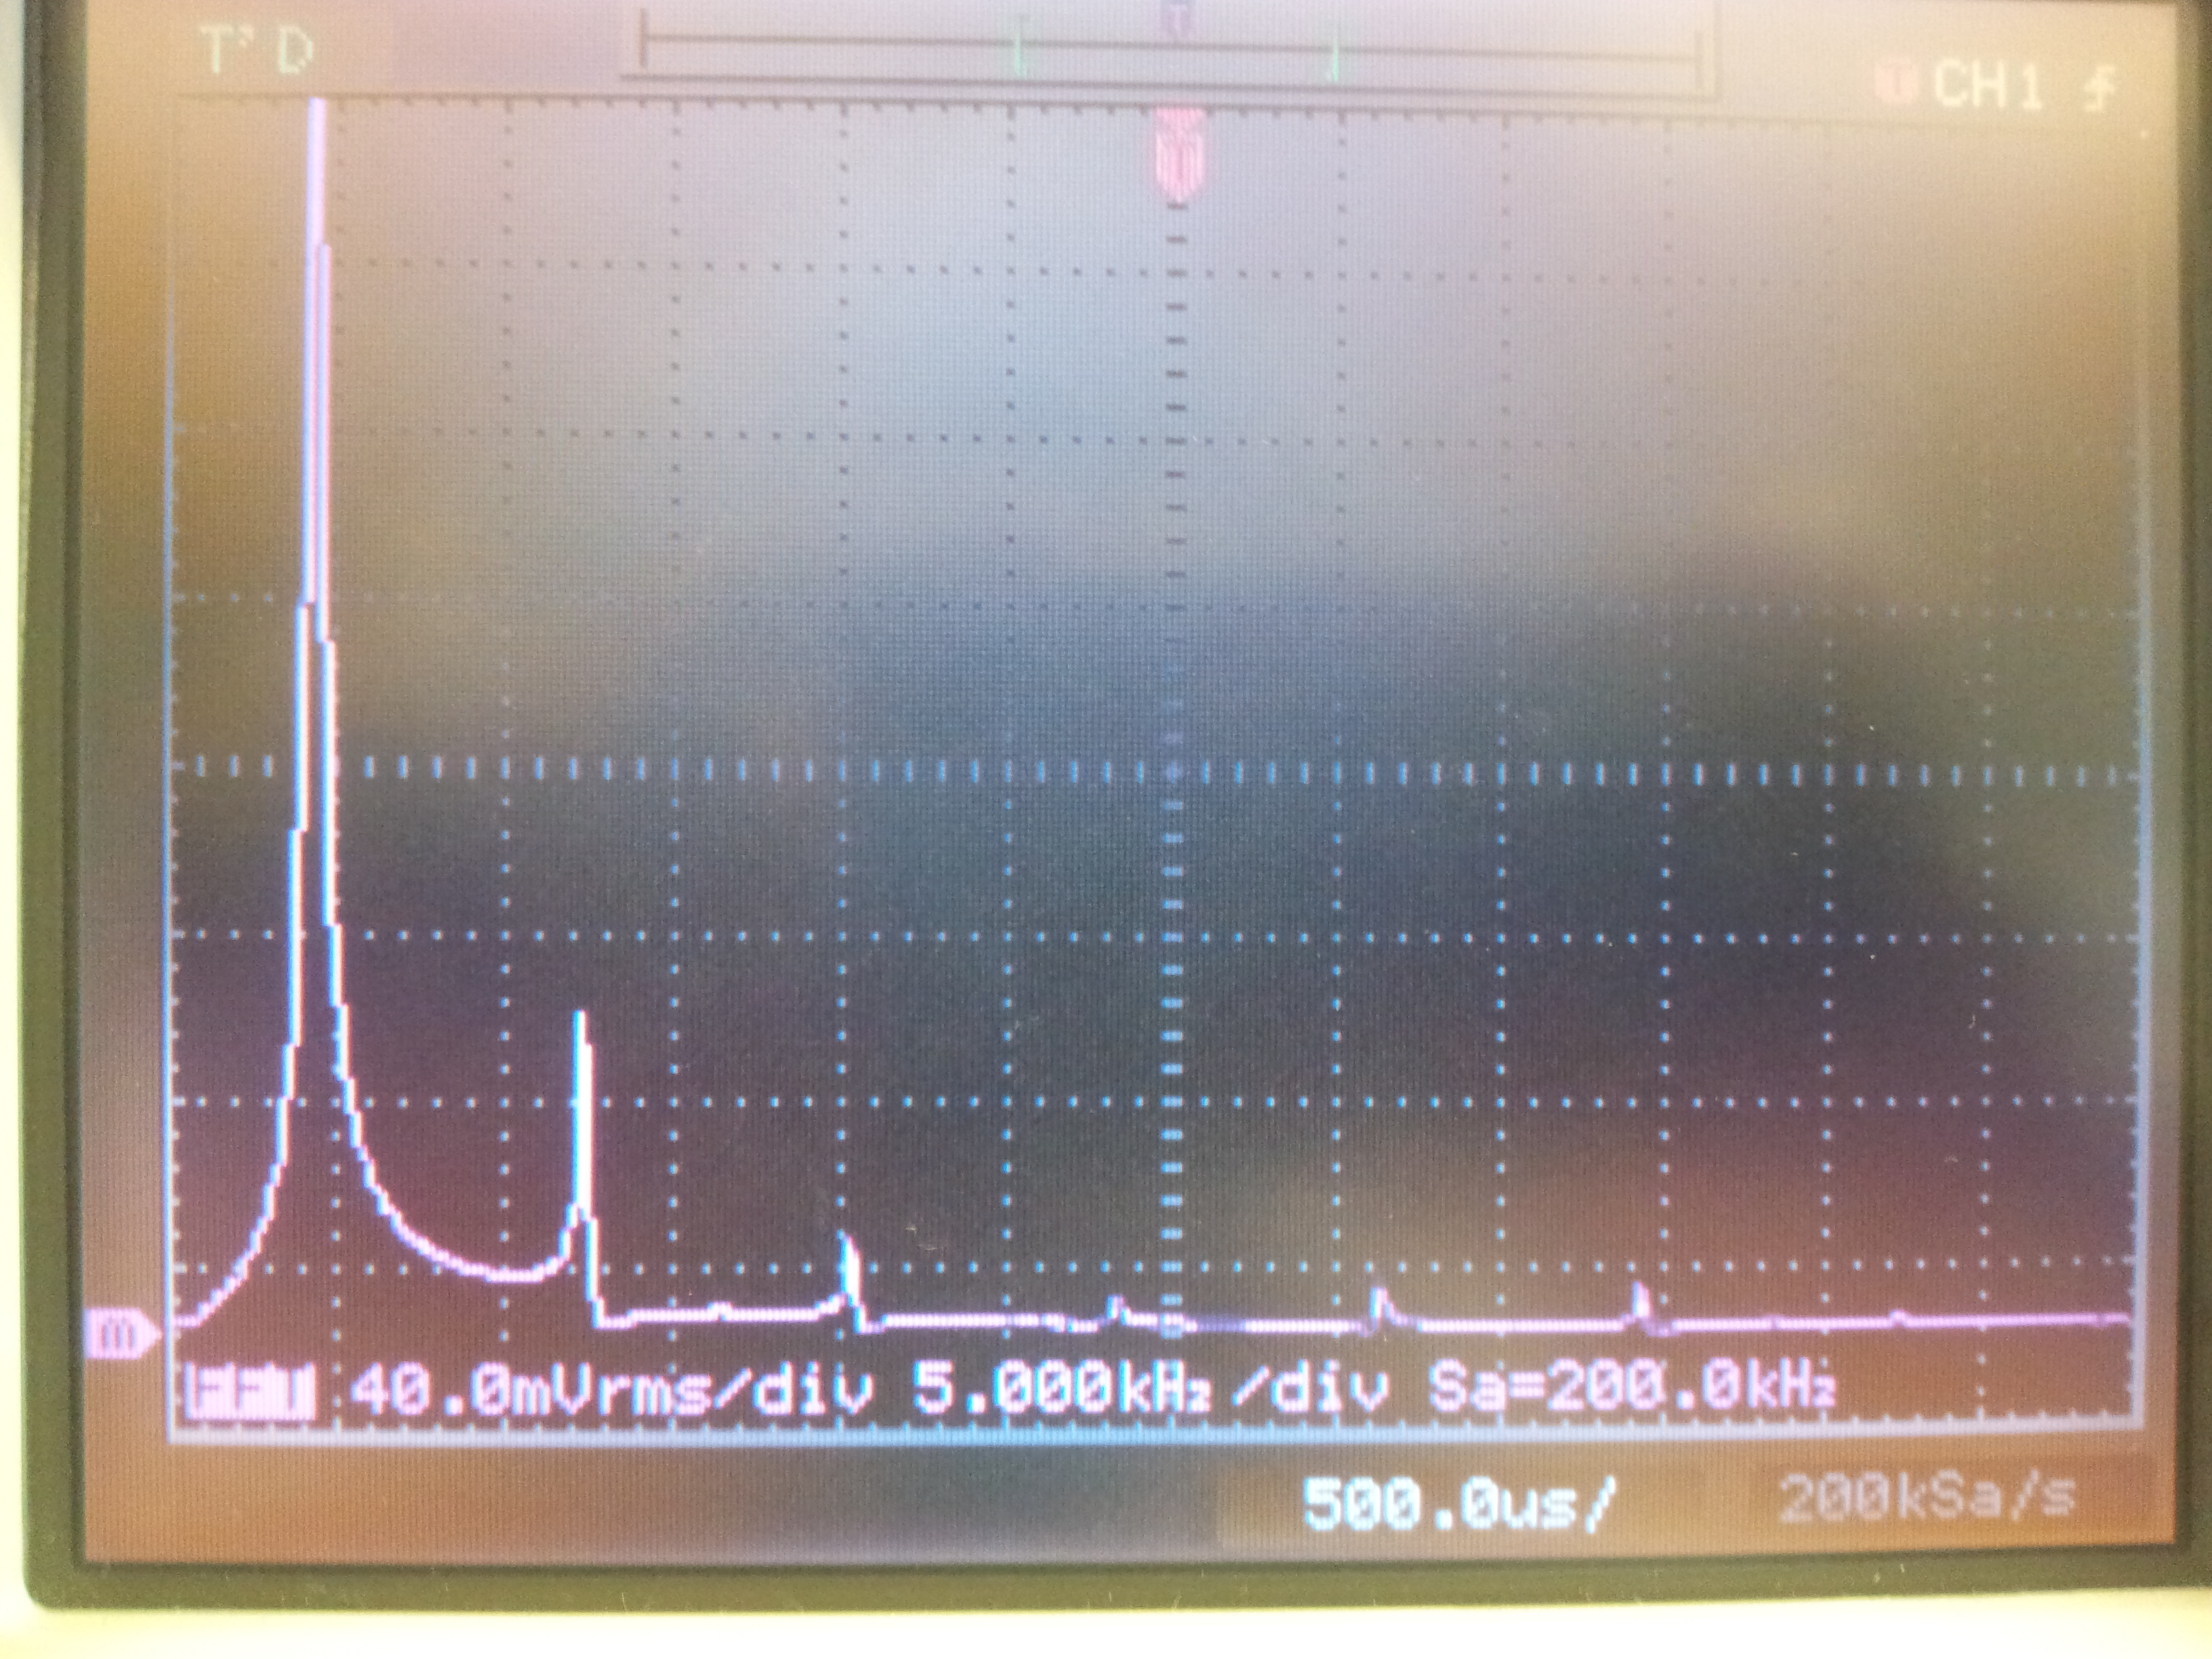
\includegraphics[width=0.5\textwidth]{./P1-8_espect_c_interp}~\\
	\caption{Espectro do sinal sinusoide com interpolação.}
	\label{fig:espect_c_interp}
\end{figure}

De novo não foi possível observar nas figuras diferenças visíveis entre os dois sinais, desta vez entre os seus espectros. Apresentam aparentemente a mesma amplitude para cada frequência entre eles mesmos.
\todo{conclusao errada, sem interp. é pior mas nao se consegue observar}
A conclusão que se pode tirar com estas observações é que o método de interpolação, embora apresente uma melhor precisão dos valores, não apresenta uma melhoria nos resultados, sendo assim um método que apenas irá exaustar mais os recursos do processador sem obter qualquer tipo de retorno notável. Podemos então concluir que caso seja preciso usar um sinal digital de uma sinusoide podemos usar apenas o método que não usa interpolação.

É importante referir que não se está a excluir a hipótese da interpolação melhorar o sinal. É afirmado que os pontos têm uma melhor precisão, mas as melhorias não são observáveis pelos métodos e equipamentos usados.

\subsubsection{P2. Transmissor BPSK}

%Introdução Teórica
O objectivo deste projeto é criar um transmissor BPSK com recurso a três elementos principais, uma fonte de bits, um codificador diferencial e mapeador, e um modulador.
Neste projeto foi utilizada uma frequência de amostragem $f_s=16$ kHz e uma frequência da portadora $f_0=4$ kHz.

\paragraph{1.Fonte de Bits} \hspace{0pt}

Para ter uma fonte de bits no transmissor usa-se um "bit-rate clock" cuja função vai ser criar uma sequência de bits $ b_n $ com $f_b=1$ kbps. Isto significa que, considerando $f_s$, a cada 16 ciclos é gerado um novo bit, alternado em relação ao anterior. Assim, implementou-se um contador que é incrementado em cada ciclo  e que tem uma condição para verificar quando chegar ao valor 16. Ao entrar nessa condição é implementada a lógica para cálculo do novo bit da sequência e o contador é reiniciado.

Para calcular o novo bit basta negar o bit anteriormente obtido de modo a obter uma sequência de bits alternada, tendo sido concretizado este raciocínio com recurso uma simples XOR:
\begin{equation}
b_n=b_{n-1} \oplus 1
\end{equation}
Com esta operação, o bit resultante será sempre alternado em relação ao anterior.
Assim, obtém-se uma onda quadrada, observada no osciloscópio, que varia entre "0" e "1" e representa $ b_n $  com uma frequência de $500$ Hz(Figura \ref{bn_cn}). Esta frequência deve-se ao fato de se dividir  $f_b$ por dois pois cada meio ciclo da onda quadrada corresponde a um bit.  

\paragraph{2.Codificador Diferencial} \hspace{0pt}

Após obter a fonte de bits passou-se ao segundo elemento do transmissor: o codificador diferencial e mapeador. Começando pelo codificador diferencial, este serve para evitar ambiguidades na fase de maneira a poder sempre recuperar uma sequência de bits num canal que tenha sofrido uma variação na fase.
A codificação de $b_n$ resulta também de uma operação lógica XOR, como se pode observar: 
\begin{equation}
c_n=c_{n-1} \oplus b_n \hspace{3 mm} ,c_0=0
\end{equation}
Como um bit novo só é calculado quando o contador chega ao valor $16$, o mesmo também só é codificado nessa condição, ou seja, a cada 16 ciclos é codificado um bit. 

Tal como em $ b_n $ também $ c_n $ é representado por uma onda quadrada que varia entre "0" e "1" só que com o dobro do período, devido a só ter dois resultados para os quatro casos possíveis da XOR que realiza a codificação(Figura \ref{bn_cn}).
\begin{figure}[H]
	\centering
	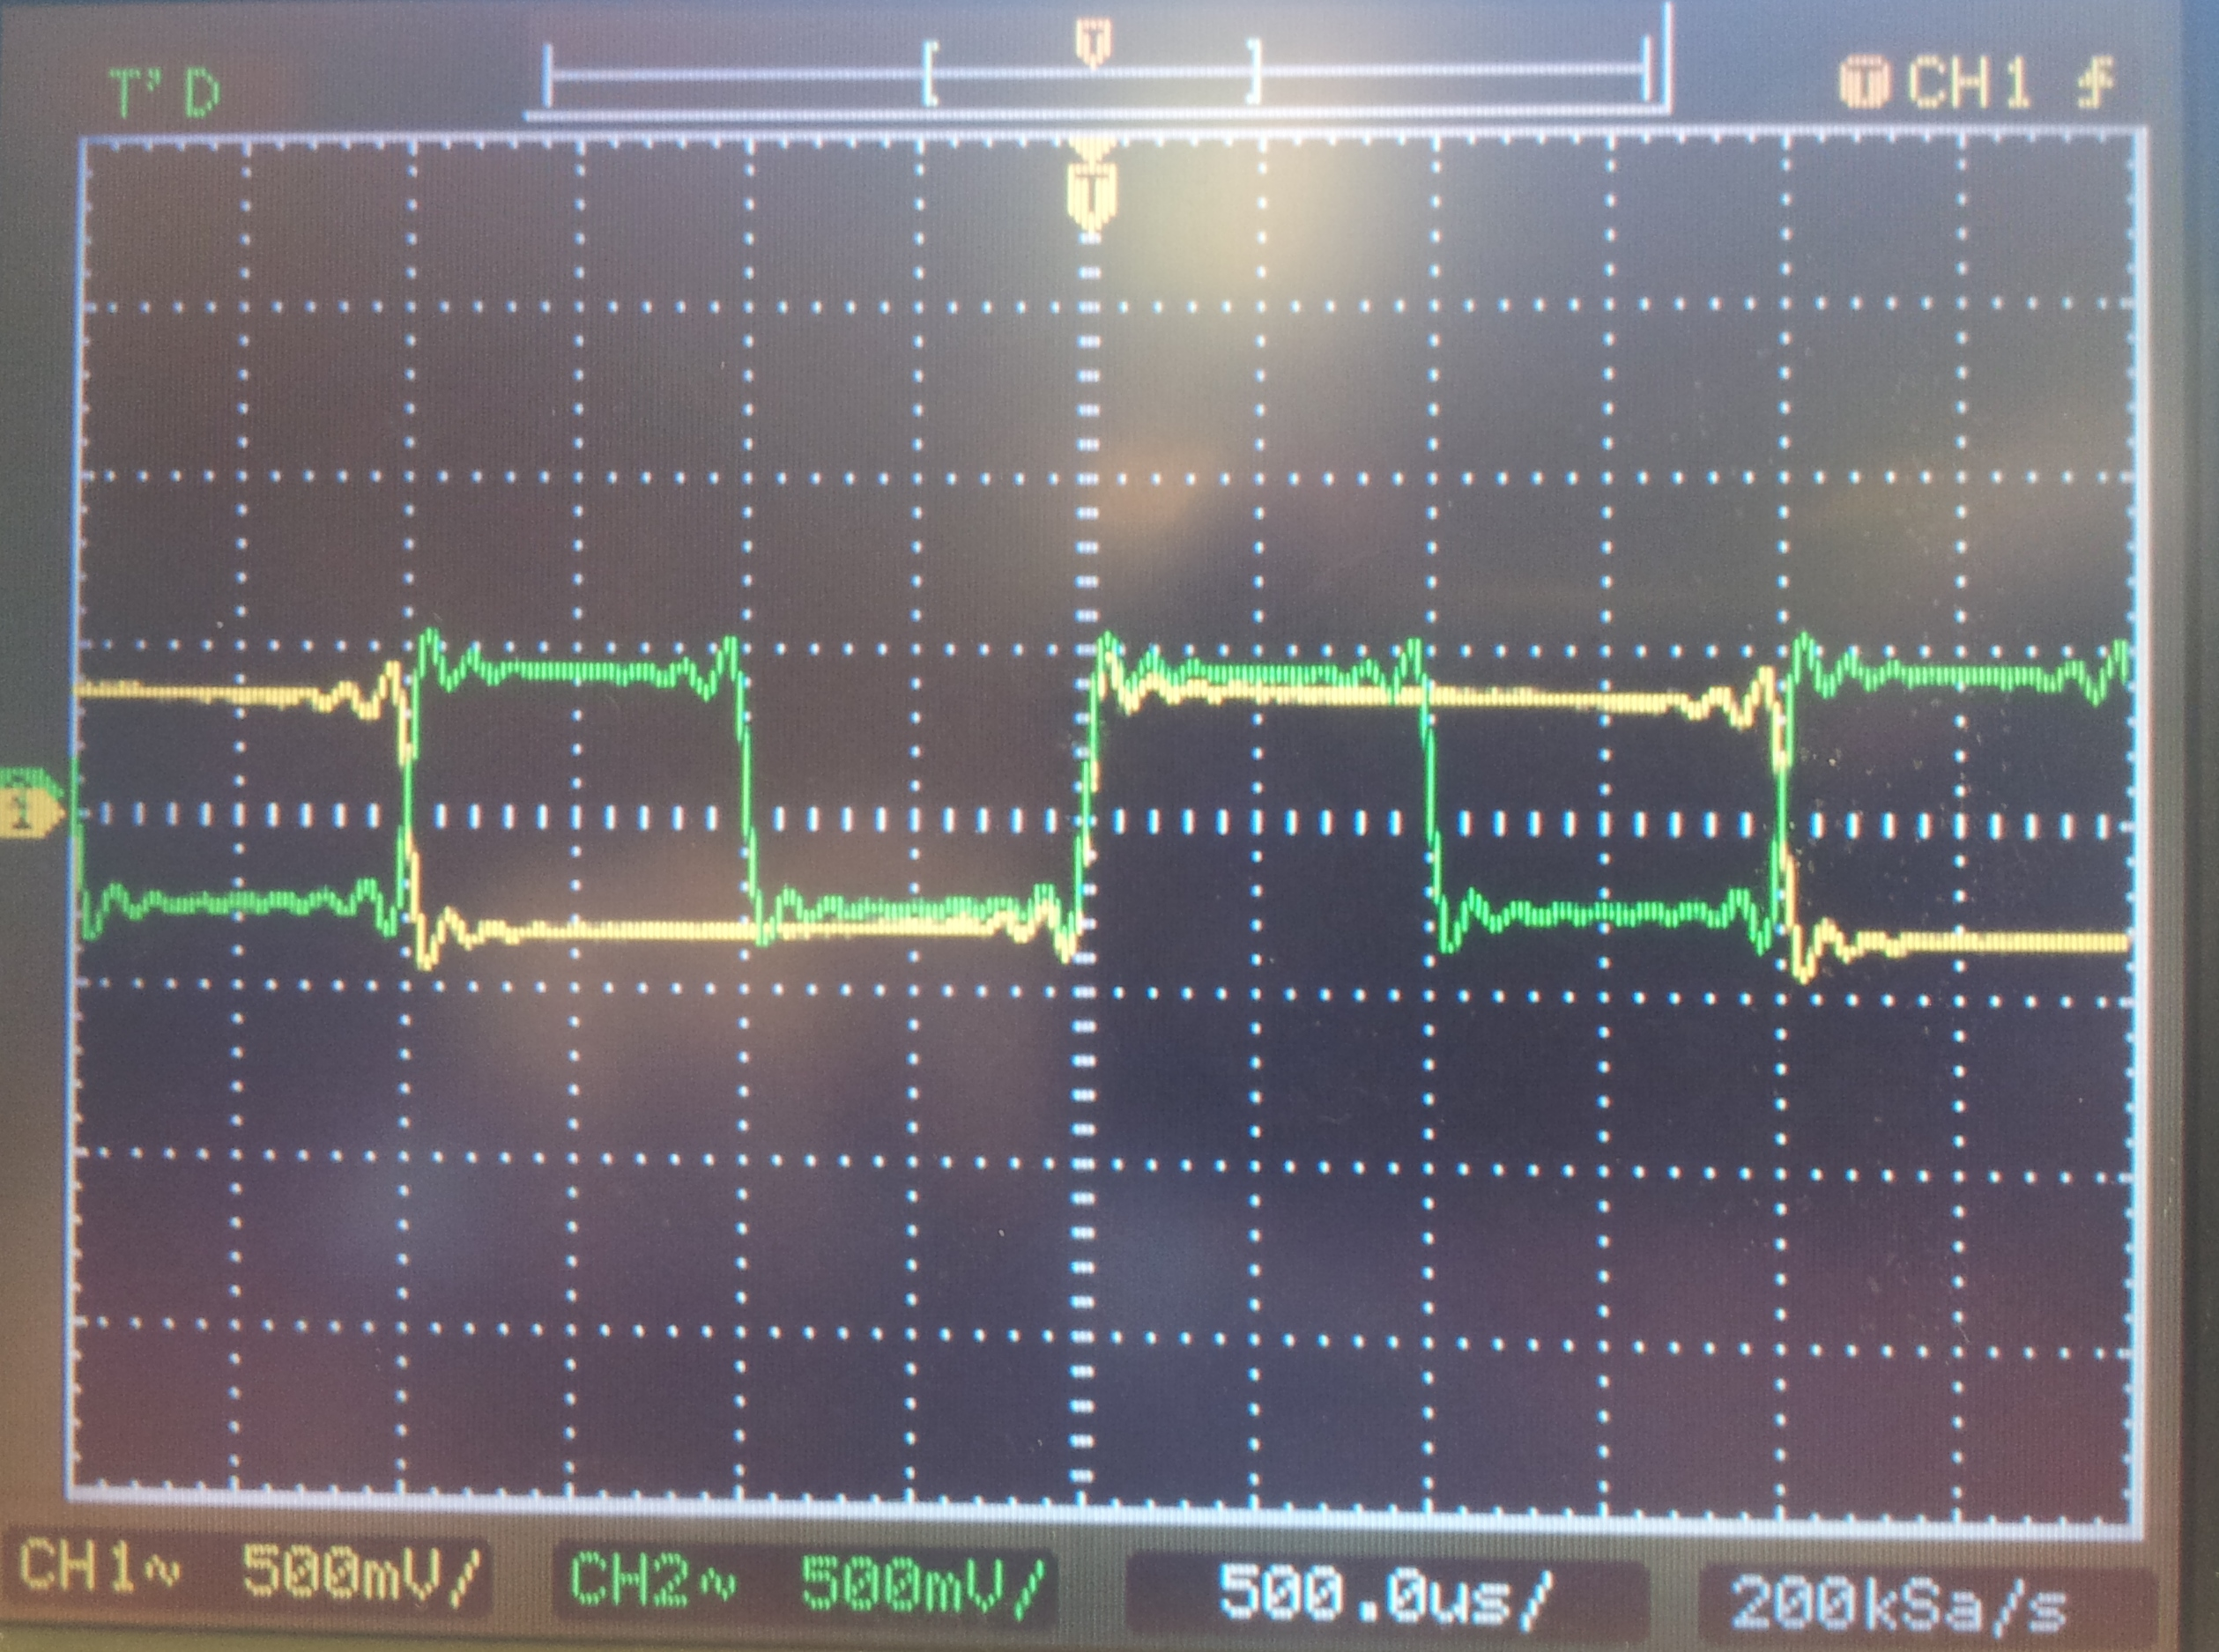
\includegraphics[width=0.5\textwidth]{./bn_cn}~\\
	\caption{$ b_n $(verde) e $ c_n $(amarelo)}
	\label{bn_cn}
\end{figure}

\paragraph{3.Mapeador} \hspace{0pt}

Depois de obter $ c_n $ passa-se ao mapeamento do mesmo. O mapeamento baseia-se em duas condições:
\begin{equation}
	c_n= '1' \rightarrow d_n =+1 \hspace{5 mm} c_n='0' \rightarrow d_n=-1
\end{equation}
Esta lógica podia ser facilmente implementada com recurso a duas condições "if", mas optou-se por evitar essa lógica para tornar o programa mais eficiente.
Assim recorreu-se a um \textit{shift} e a uma subtração. Atenção que esta não é a maneira mais eficiente pois a subtração faz com que o programa tenha de passar pela ALU.
Pode-se observar então o mapeamento efetuado através da seguinte expressão:
\begin{equation}
d_n=32767*((c_n << 1)-1)
\end{equation}
Antes de mais, o ganho que está a ser multiplicado é utilizado para converter o resultado em Q15, como já foi feito anteriormente. Considerando a expressão sem esse ganho, vê-se que para $ c_n=0 $, como o \textit{shift} não influencia o resultado, o mesmo só depende da subtração e é sempre o pretendido, $d_n=-1$. Se $c_n=1$, o \textit{shift} duplica  esse valor, e depois ao subtrair obtém-se $d_n=1$.

Tal como em $b_n$ e $c_n$ esta operação só é executada a cada 16 ciclos pois depende diretamente de $c_n$ e só se mapeia um novo bit depois de ele ser codificado. Concluído o mapeamento obtém-se mais uma vez uma onda quadrada mas desta vez varia entre "-1" e "1" (figura \ref{cn_dn}).
\begin{figure}[H]
	\centering
	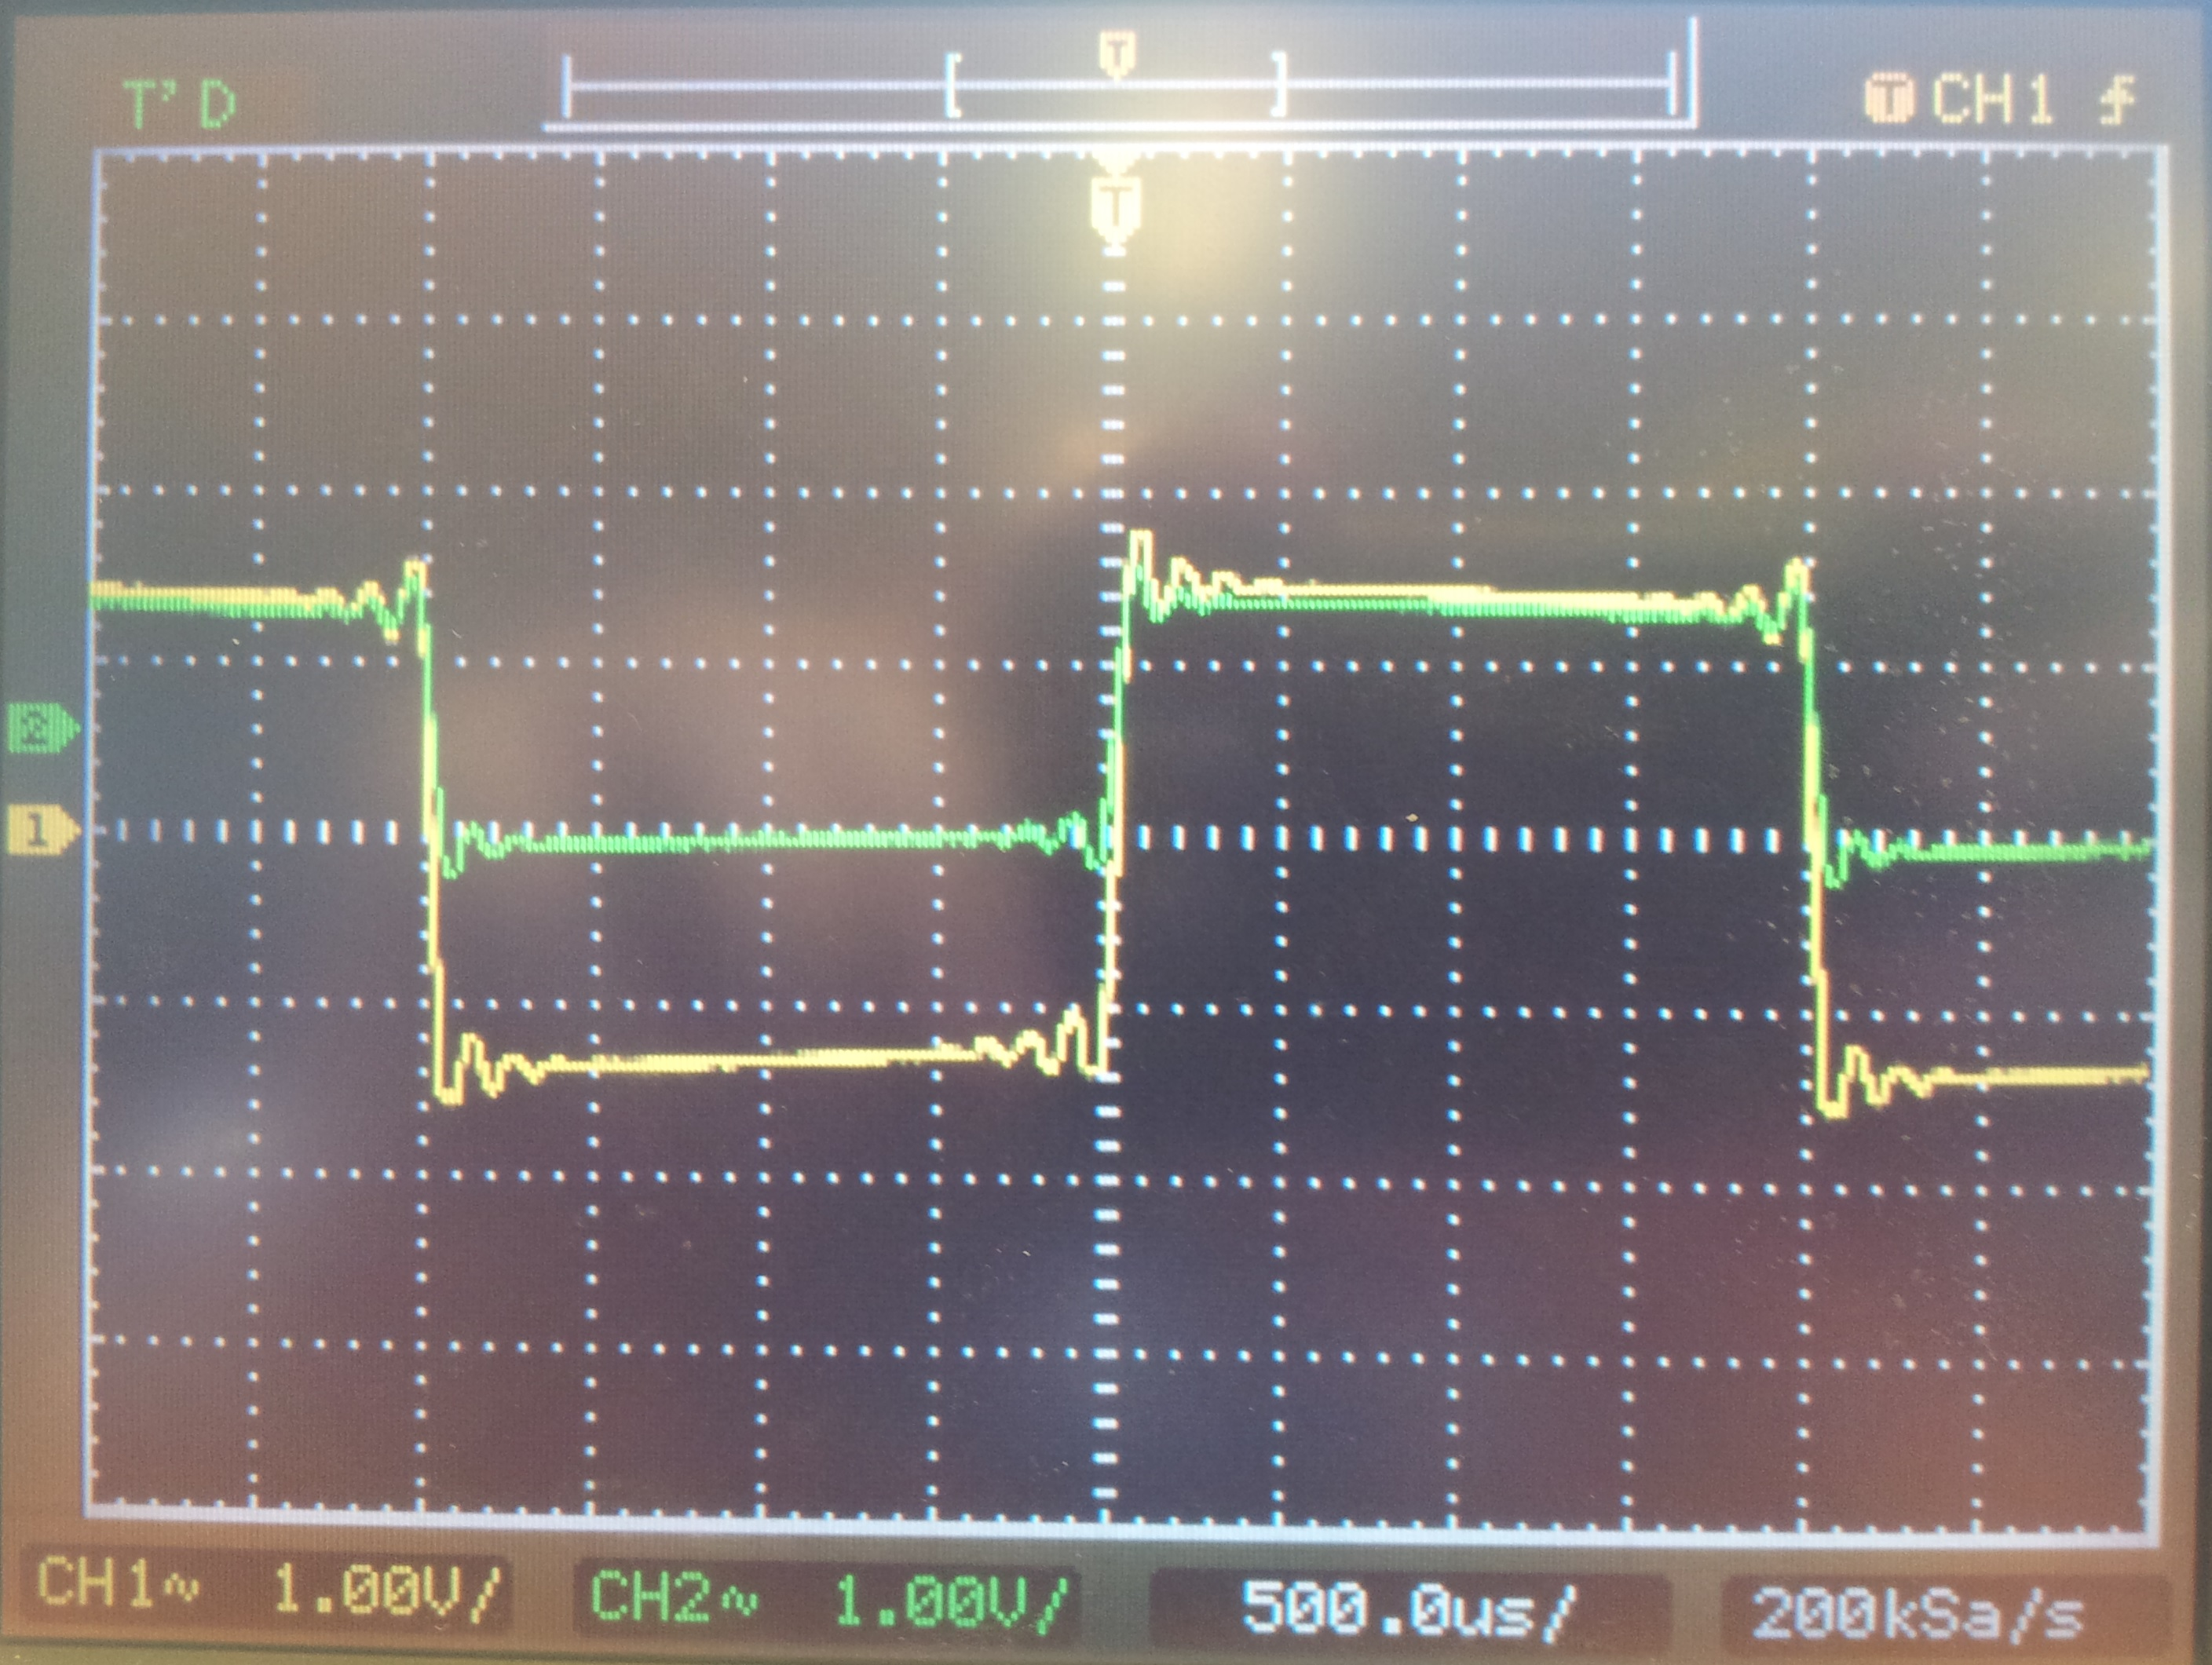
\includegraphics[width=0.5\textwidth]{./cn_dn}~\\
	\caption{Formas de onda de $d_n$ (amarelo) e $c_n$ (verde).}
	\label{cn_dn}
\end{figure}                                                                                                                                     
                                                                              
\paragraph{4.Implementação do Modulador} \hspace{0pt}

Falta agora gerar a onda portadora a modular. Esta foi implementada de forma mais simples face ao projeto anterior uma vez que a frequência é constante (4 kHz) e este valor consiste numa fração inteira da frequência de amostragem ($16 kHz$).
Em primeiro lugar criou-se uma tabela com quatro valores dum período da sinusóide, sendo esta:
\begin{table}[H]
	\centering
	\caption{Amostras da onda portadora}
	\label{tab:amostras}
	\begin{tabular}[c]{|l||c|}
		\hline \textbf{contador} & \textbf{seno}\\ 
		\hline $ 0 $ & $ 0 $\\ 
		\hline $ 1 $ & $ 32767 $  \\ 
		\hline $ 2 $ & $ 0 $ \\ 
		\hline $ 3 $ & $ -32767 $ \\
		\hline
	\end{tabular}
\end{table}
Escolheram-se estes valores uma vez que o período de amostragem coincide com os instantes de máximo, mínimo e \textit{zero-crossing} da portadora. Para gerar a portadora (Figura \ref{port_mod}) recorreu-se a um contador que, em cada interrupção (ocorrendo em cada instante de amostragem, como explicado no enunciado), aponta para cada entrada da tabela e põe a amostra numa variável que, após se incrementar o contador, irá ser multiplicada por $d_n$. Esta tabela não gera uma onda triangular pois das harmónicas destas, abaixo da frequência de amostragem ( $f_0$=4kHz e 3$f_0$=12kHz) apenas a primeira harmónica se encontra na banda de passagem do filtro de reconstrução do DAC, que terá frequência de corte Fs/2.

A onda modulada é então representada pela seguinte expressão:
\begin{equation}
	s_n= d_n \sin(2 \pi f_0T_sn) 
\end{equation}
Neste caso os valores do seno são os valores das amostras discutidas anteriormente.
\vspace{2 mm}
                                              
\paragraph{5.Teste do Modulador BPSK} \hspace{0pt}

Após implementar o modulador, tem-se o transmissor BPSK completo e para testá-lo, pôs-se nos dois canais do osciloscópio a onda portadora e a onda modulada (Figura \ref{port_mod}).
\todo{trocar imagem pela q tem mais transições}
\begin{figure}[H]
	\centering
	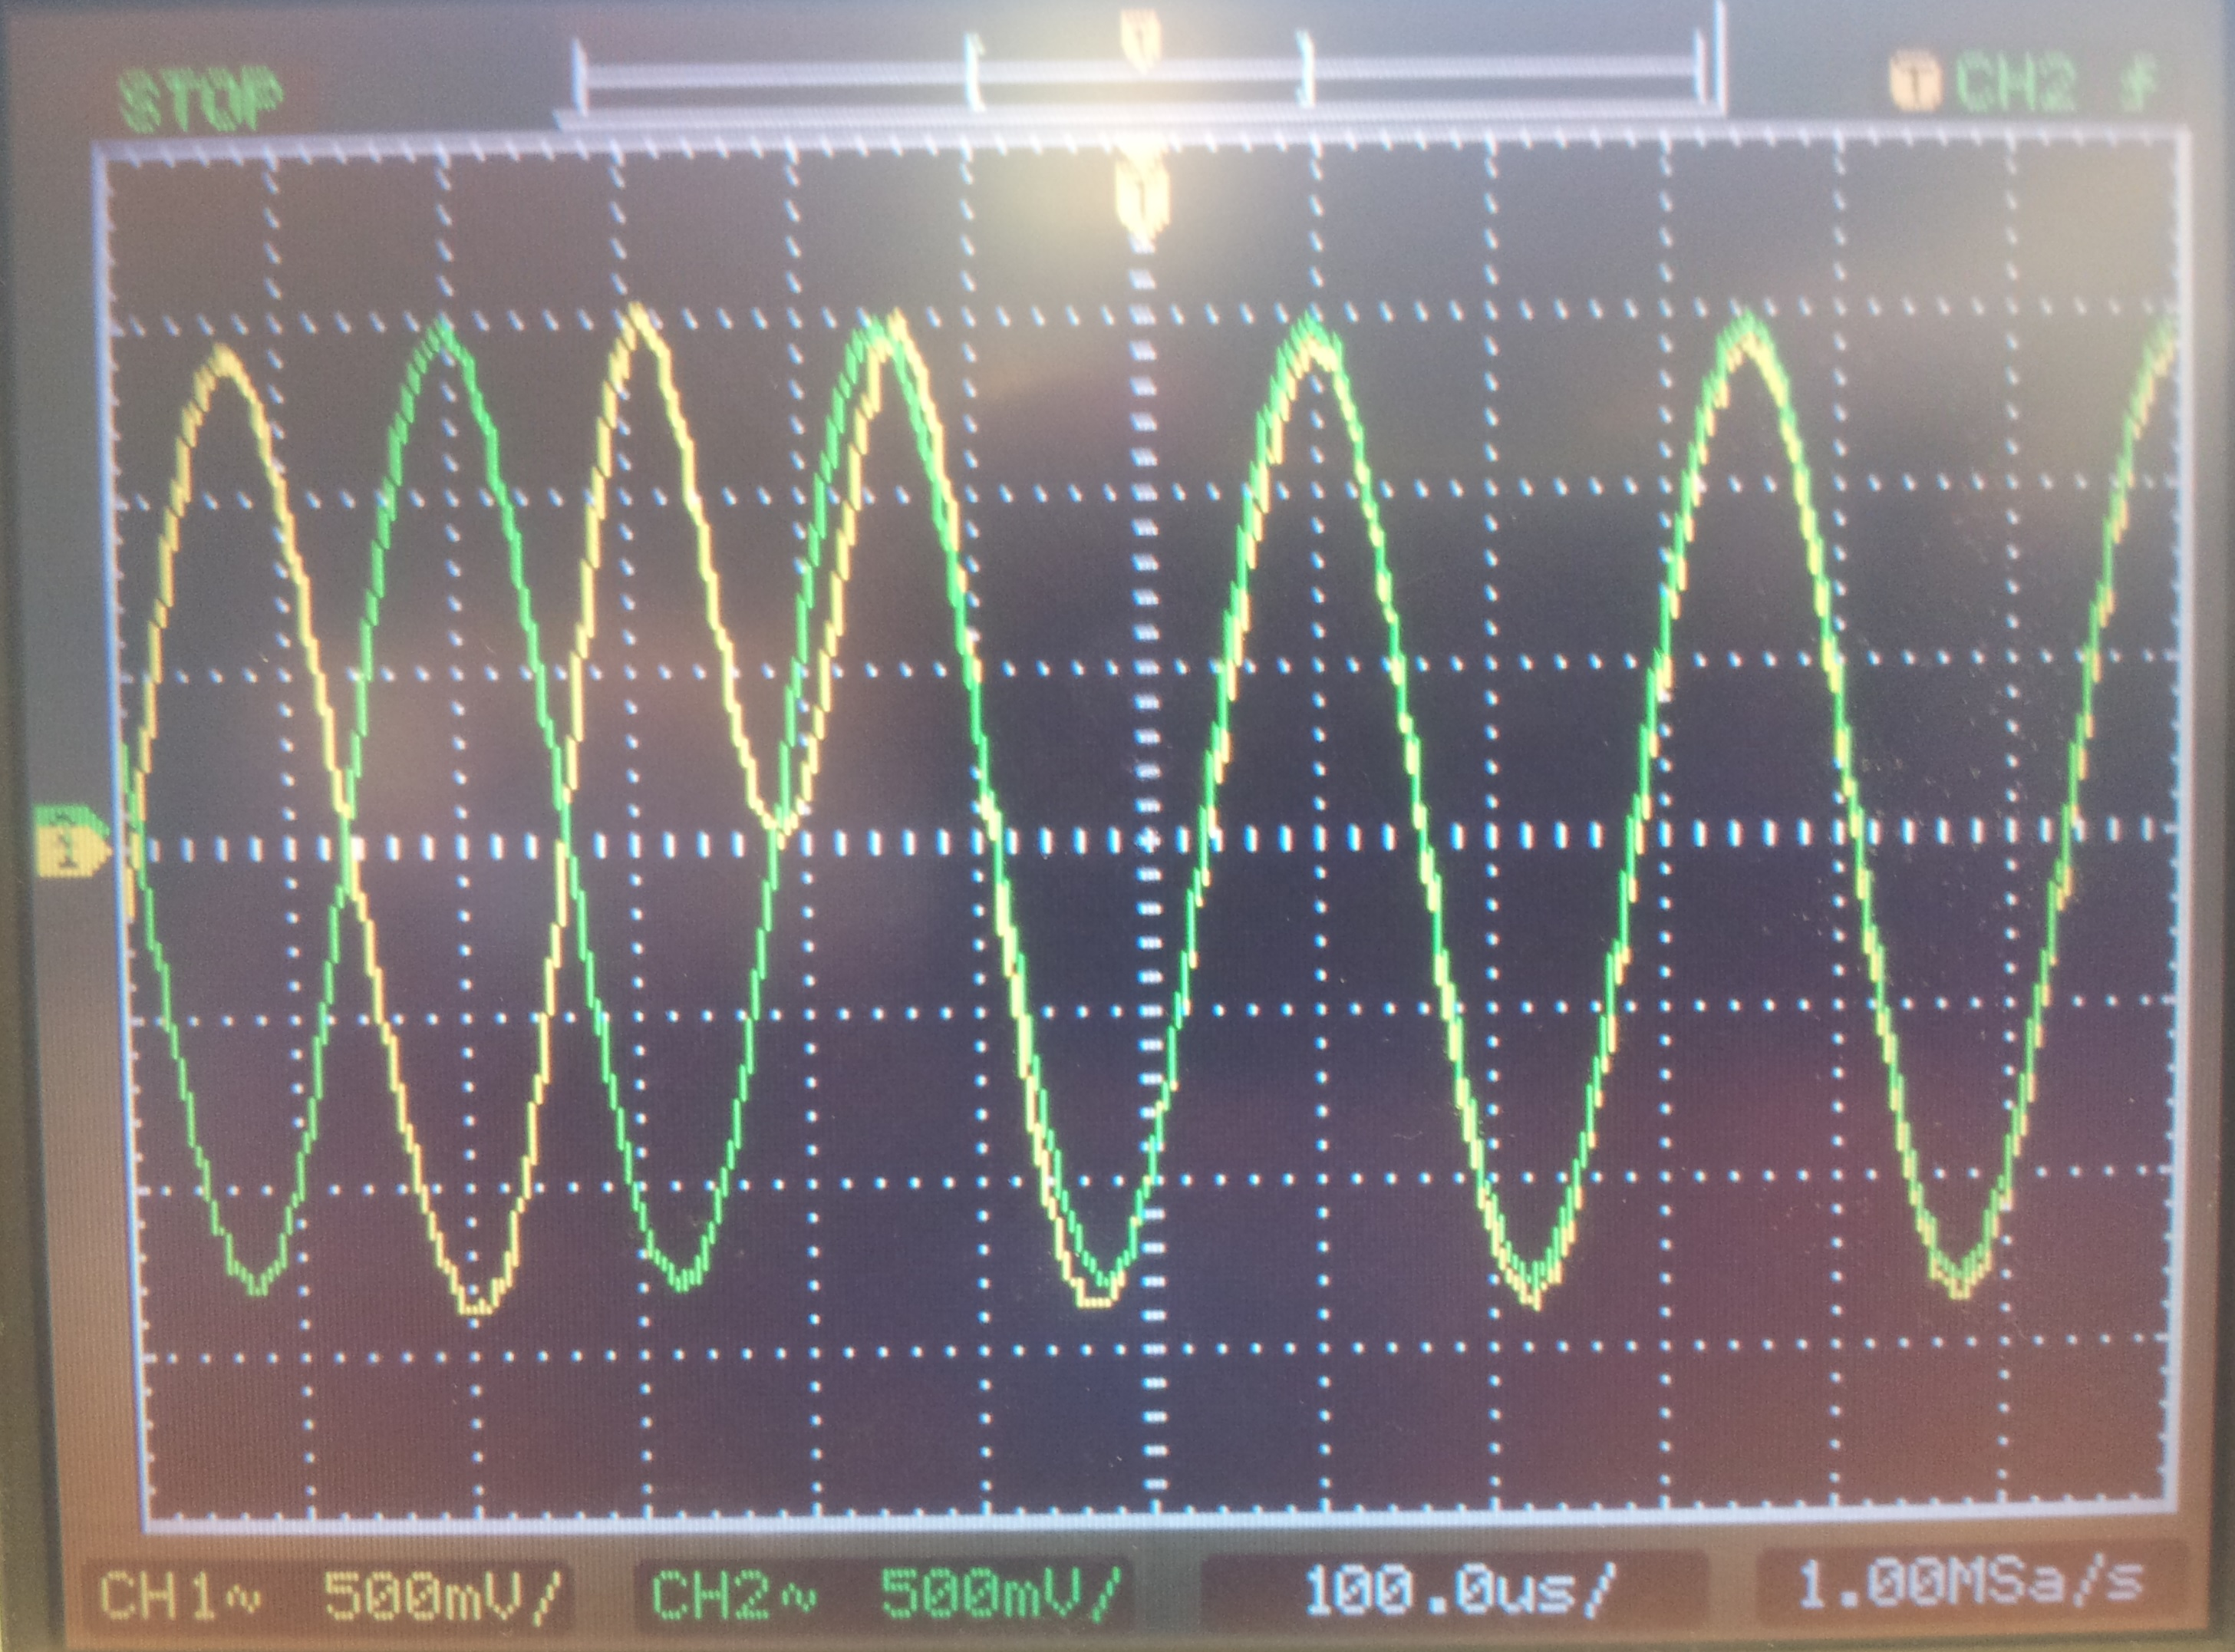
\includegraphics[width=0.5\textwidth]{./port_mod}~\\
	\caption{Onda portadora (verde) e onda modulada (amarelo)}
	\label{port_mod}
\end{figure} 
 \vspace{2 mm}
 
 Como se pode observar pela imagem e considerando a expressão (8), a onda portadora começa em oposição de fase com a onda modulada. Isto ocorre quando $d_n=-1$, o que significa que quando $d_n=1$ a onda modulada é igual à portadora. É possível observar quando $d_n$ muda de valor pois é exatamente quando a onda modulada inverte a sua fase (Figura \ref{dn_mod}). 
 
 
 \begin{figure}[H]
 	\centering
 	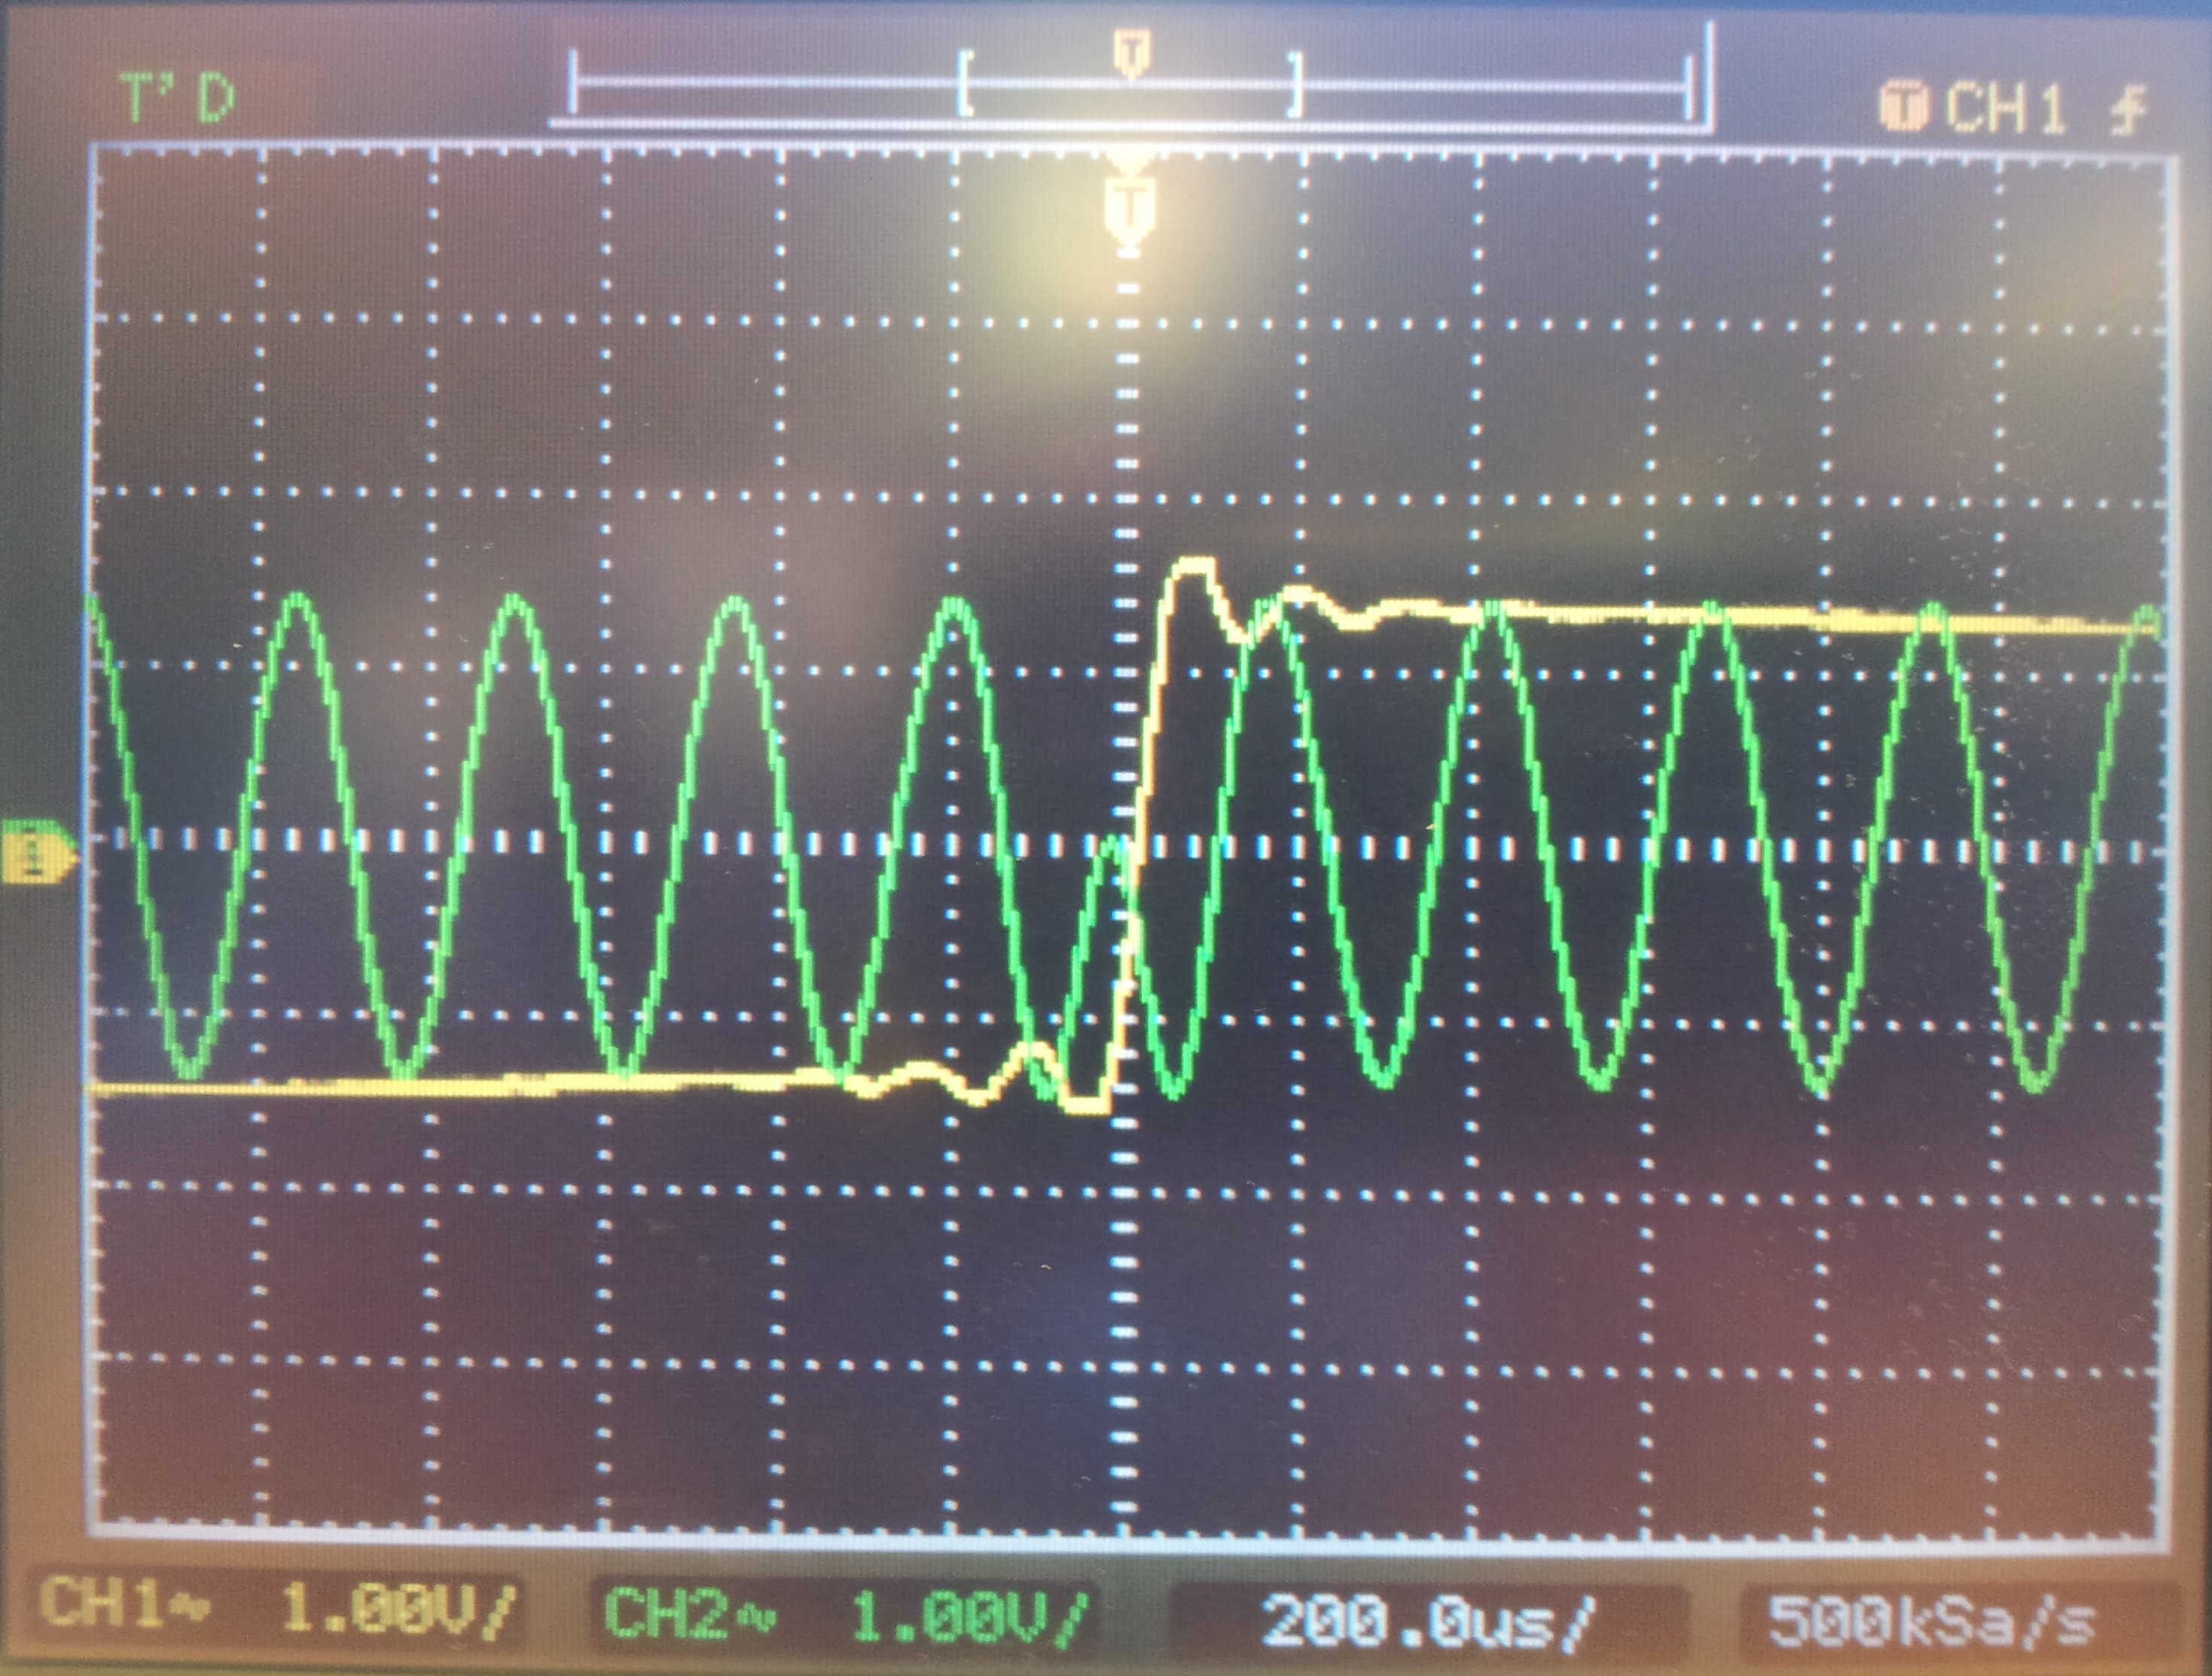
\includegraphics[width=0.5\textwidth]{./dn_mod}~\\
 	\caption{Formas de onda de $d_n$ (amarelo) e $s_n$ (verde).}
 	\label{dn_mod}
 \end{figure}
 Este fenómeno acontece a cada 8 ciclos pois, como já foi explicado anteriormente, a frequência da onda correspondente à fonte de bits é o bit-rate dividido por dois e uma vez que a codificação divide esta frequência por dois, ou seja, a frequência de $d_n$ é 250 Hz e por isso cabem oito ciclos da portadora num meio ciclo de $d_n$.
 \vspace{2 mm}

\paragraph{6.Espectro do Sinal Modulado} \hspace{0pt}
Para compreender melhor o sinal modulado, observou-se o espetro do mesmo (Figura \ref{espetro}).
\begin{figure}[H]
	\centering
	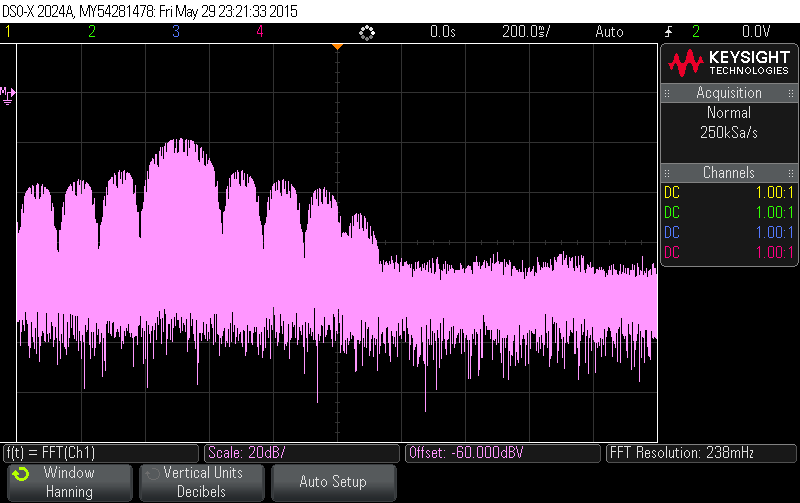
\includegraphics[width=0.5\textwidth]{./spectrum_sn_0-16k}~\\
	\caption{Espectro do sinal $s_n$.}
	\label{espetrosn}
\end{figure}
A onda modulada no tempo consiste na multiplicação de uma onda quadrada com uma onda sinusoidal, na frequência isto consiste na convolução do espetro da primeira, um $sinc$, com o espetro da segunda, um impulso em $f_0$. Isto resultaria numa translação do espetro da onda quadrada, ficando centrado na frequência da onda sinusoidal.

Na imagem acima vê-se o espectro de $d_n$ centrado em 4kHz como esperado. O espetro tem o \textit{SPAN} [0-16KHz] e apresenta a forma descrita acima, exceto a falta de réplica a 16kHz, contudo isso é explicado pelo filtro anti-aliasing do analisador de espetros.

consiste na convolução do espetro da primeira (impulsos nos múltiplos ímpares da frequência fundamental) com o espetro da segunda (um impulso à frequência $f_0$). Isto resultaria numa translação do espetro da onda quadrada, ficando centrado na frequência da onda sinusoidal.

Na imagem acima vê-se o espectro de $d_n$ centrado em 4kHz como esperado. Como se pode observar, as harmónicas de maior amplitude estão espaçadas 250 Hz em relação a $f_0$ indicando que a frequência fundamental da onda quadrada é 250 Hz, como esperado.

\subsubsection{Receptor \textit{Costas Loop}}
\todo{introdução teorica}
%Quem vai fazer o guilherme?
Para um bom funcionamento do bloco total é necessário um \textit{scrambler} cuja função é

%Nome melhor para bloco total teorica}

\paragraph{1.Introdução do \textit{Scrambler}:} \hspace{0pt}

\todo{guilherme}
Para um bom funcionamento do bloco total é necessário um \textit{scrambler} cuja função é

%Nome melhor para bloco total
\paragraph{2.Implementação de NCO controlado pelo erro:} \hspace{0pt}

\todo{joao}
Para implementar o NCO controlado pelo erro, recorreu-se ao NCO implementado na secção \ref{NCO}, com a mesma rampa, LUT e indexação da mesma como se pode ver no código seguinte.
\begin{lstlisting}
	rampa=rampa+delta;
	index=rampa>>10;
	index=31 & index;
	aux=ampl*LUT[index];aux=aux<<1;
\end{lstlisting}
Mas agora falta a parte de controlar o NCO com o erro. Este controlo da frequência é feito da mesma maneira que na secção \ref{NCO}, através da variável delta (equação \ref{delta}), este controlo observa-se na linha de código a seguir.
\begin{lstlisting}
  delta=16384+(erro>>2);
\end{lstlisting}
Assim, como o erro controla delta e este controla a rampa que indexa a LUT obtém-se um NCO controlado pelo erro.
A seguir prosseguiu-se à obtenção das componentes em fase e em quadratura do sinal pretendido. A componente em fase já tinha sido obtida anteriormente na secção \ref{NCO} pois corresponde ao sinal sinusoidal (figura \ref{quad}). Como a LUT corresponde a meio ciclo do seno foi necessário implementar uma pequena lógica para criar a outra metade do ciclo, enunciada no código a seguir.
\begin{lstlisting}
	if(rampa<0)  seno=-aux>>16;
	else seno=aux>>16;
\end{lstlisting}
Assim, tem-se duas zonas identificadas pelo sinal da rampa, o meio ciclo positivo e o meio ciclo negativo do seno.
No caso da componente em quadratura, devido ao \textit{offset} de 16 amostras obtém-se um sinal coseno. Este não é tão fácil de representar como o seno, desta vez é necessário ter em conta 4 situações, 4 zonas diferentes num ciclo. Nestas zonas o que varia é a secção da LUT que é indexada e o sinal do coseno, que dependem do sinal da rampa e da secção da LUT que estiver a ser indexada para o seno. Estas zonas estão enunciadas nos códigos seguintes.
\vspace{1mm}

\textbf{1ª zona}
\begin{lstlisting}
	if(rampa<0){
	  if(index<=15){
	    aux=ampl*(-LUT[(index+16) & 31]);aux=aux<<1;
	  }coseno=aux>>16;
	}
\end{lstlisting}
A primeira zona do ciclo do coseno corresponde quando a rampa é negativa e o seno está a descer do zero ao seu mínimo (-32767), ou seja, quando se indexa a primeira metade da LUT com o sinal invertido. Assim, quando o seno tem esse comportamento, o coseno está a subir do seu mínimo ao zero, sendo necessário aplicar um \textit{offset} positivo de 16 amostras, ou seja, indexar a segunda metade da LUT, também com o sinal invertido. Foi aplicada uma máscara com 31 de modo ao \textit{offset} nunca causar um índice superior ao permitido na LUT, 31.
\vspace{1mm}

\textbf{2ª zona}

Esta zona também só existe quando a rampa é negativa. No código seguinte pode-se observar o raciocínio implementado para a mesma.
\begin{lstlisting}
	else{
	  aux=ampl*(LUT[(index-16) & 31]); aux=(aux<<1);
	}coseno=aux>>16;
\end{lstlisting}
Continuando o comportamento do seno, este vai subir do mínimo ao zero,ou seja, indexa a segunda metade da LUT mais uma vez com o sinal invertido. Logo, o coseno sobe do zero ao máximo (32767) o que implica um \textit{offset} negativo de 16 amostras para indexar a primeira metade da LUT, sem inverter o sinal.

Para a terceira e quartas zonas efetua-se o mesmo raciocínio de indexação só que só se inverte o sinal da LUT na quarta zona pois nestas a rampa é positiva.
\vspace{1mm}

\textbf{3ª zona}
\begin{lstlisting}
	if(index<=15){
	  aux=ampl*LUT[(index+16) & 31];aux=aux<<1;
	}coseno=aux>>16;
\end{lstlisting}
Aqui, o seno vai subir do zero ao máximo, ou seja, primeira metade da LUT, logo, como o coseno vai descer do máximo ao zero, interessa aceder à segunda metade da LUT, aplicando um \textit{offset} positivo de 16 amostras.
\vspace{1mm}

\textbf{4ª zona}
\begin{lstlisting}
	else{
	  aux=-ampl*LUT[(index-16) & 31];aux=aux<<1;
	}coseno=aux>>16;
\end{lstlisting}
Por fim, chega-se à última zona do ciclo, onde o seno volta ao zero a partir do máximo, ou seja, segunda metade da LUT. Como o coseno volta ao mínimo a partir do zero, aplicando um \textit{offset} negativo de 16 amostras e uma inversão de sinal nas posições indexadas pela LUT.

Assim obteve-se o sinal em quadratura (figura \ref{quad}).
\begin{figure}[h]
	\centering     
	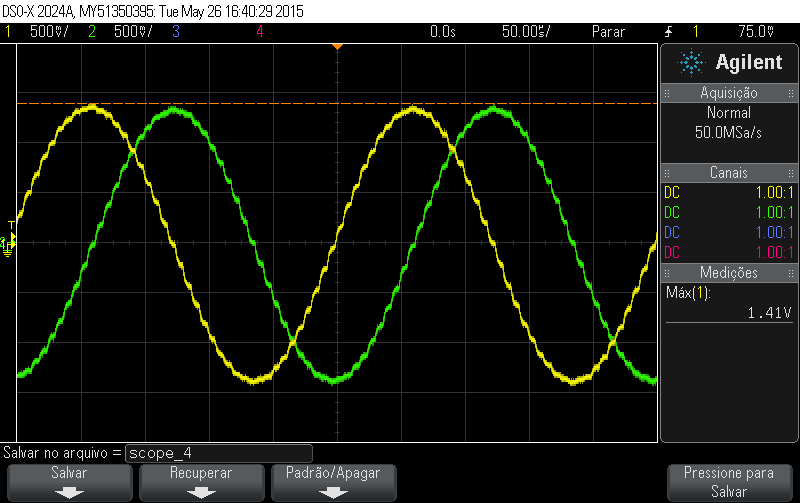
\includegraphics[width=0.6\textwidth]{./quadratura}~\\
	\caption{Componentes e fase(verde) e em quadratura do sinal(amarelo).}
	\label{quad}
\end{figure}
Como se pode observar ao comparar as duas componentes verifica-se qu estão desfasados por um quarto de ciclo, o que significa um offset de 16 amostras.
\paragraph{3.Implementação dos Filtros:} \hspace{0pt}                                                                                                                                                                                                              durante
\todo{guilherme}

\paragraph{4.\textit{Loop} desmodulador:} \hspace{0pt}
  \todo{rever a linguagem}
 
%misturado? Queria dizer "passar pelo scrambler", pensei scrambled => misturado. Mas se nao ficar claro muda-se
Nesta fase do projeto têm-se todos os blocos necessários do modem BPSK. O sinal de informação $b_n$ foi misturado, $e_n$, codificado e mapeado, $d_n$, e posteriormente multiplicado à portadora com frequência $f_0 = 4kHz$, obtendo o sinal modulado BPSK, $s_n$. Este durante a transmissão pode sofrer variações de fase ($\Delta\phi=\phi_0-\phi_1$) e de frequência ($\Delta f = f_1-f_0$) tomando a forma:
\begin{equation}
	s_n=d_nsin(2\pi f_1t+ \phi_1)
\end{equation}
 Para o desmodular é necessário sincronizar o oscilador local com a frequência da portadora, estimando $\Delta\phi$ e $\Delta f$.

Usa-se, então, o \textit{Costas Loop}, um tipo de PLL. Em semelhança aos seus familiares é composto por um detetor de fase, um \textit{loop filter} e um oscilador local(NCO), excepto nos dois filtros adicionais em cada ramo exterior. No braço inferior o sinal BPSK é multiplicado com o sinal $cos(2\pi f_0t+\phi_0)$ e no superior com $sin(2\pi f_0t+ \phi_0)$ obtendo-se a componente em quadratura e fase do sinal $s_n$, respectivamente: 
\begin{equation}
s_1=\frac{d_n}{2}[cos(4\pi f_0t+\Delta f+\phi_1+\phi_0)+cos(\Delta f+\phi_0-\phi_1)]
\end{equation}
\begin{equation}
s_2=\frac{d_n}{2}[sin(4\pi f_0t+\Delta f+\phi_1+\phi_0)+cos(\Delta f+\phi_0-\phi_1)]
\end{equation} 

Nestes dois multiplicadores ocorre a detecção de fase uma vez que os termos de baixa frequência têm como componentes $\Delta\phi$ e $\Delta f$, os indicadores dos erros de fase e frequência que se usará no NCO. Filtrando-se esses sinais nos \textit{Data filters}, multiplicando-os entre si e passando no \textit{Loop filter} obtém-se 
\begin{equation}
\epsilon(t)=\frac{1}{8}sin(2\Delta\phi)\approx\frac{1}{4}\Delta\phi
\end{equation}


para valores pequenos de $\Delta\phi$. Este sinal estático entra no NCO e aumenta ou diminui a frequência do oscilador reduzindo por consequência o $\Delta f$, desde que a frequência da portadora se encontre na banda de captura do dispositivo descrito.

Uma vez capturada a frequência da portadora (diferente da frequência central) o oscilador local encontra-se sincronizado à frequência da portadora ($f_1 = f_0+\Delta f$) e em fase com a mesma ($\Delta\phi=0$) tendo-se os sinais
\begin{equation}
\frac{1}{2}d_ncos(\Delta\phi)\approx\dfrac{d_n}{2} \hspace{1mm}, \hspace{1mm} \frac{1}{2}d_nsin(\Delta\phi)\approx 0
\end{equation}
à saída do filtro da componente em quadratura e do filtro da componente em fase, respetivamente, tornando-se o braço do primeiro num detetor coerente. Como já mencionado, o espetro do sinal BPSK é o espetro do sinal de informação centrado à frequência da portadora e quando se multiplica pelo sinal local sincronizado obtêm-se réplicas do espetro do sinal de informação a $f=0$ e $f=2f_1$, que ao passar no \textit{Data filter} filtra as componentes superiores a 1kHz obtendo o sinal de informação.


\paragraph{5.Testes do \textit{Costas Loop} com onda sinusoidal} \hspace{0pt}

\todo{joao}
%ondas sinusoidais usadas no gerador do osciloscopio
%bandas de captura e seguimento upper arm
%frequencia central 4kHz
%bandas de captura e seguimento Costas Loop
%complementar com codigo relacionado

\paragraph{6.Testes do \textit{Costas Loop} com BPSK sem zero}
%sinal modulado na entrada
%diferenças no codigo
%resultado do sinal desmodulado, o q melhorar e como o fazer
%comparaçao com dn, aleatoridade devido a en
\todo{Joao}

\paragraph{7.Testes do \textit{Costas Loop} com BPSK com zero} \hspace{0pt}

O sinal obtido do \textit{Costas Loop} ainda apresenta um vestígio da multiplicação no detetor de fase, sendo possível observar-se uma oscilação de maior frequência somada ao sinal de informação. Tal é devido ao aliasing existente nos filtros discretos que, dadas as réplicas espectrais somarem o ganho no limite de Nyquist, $\frac{F_s}{2} = 8kHz$, o filtro  não é seletivo que chegue a essa frequência resultando no observado na figura acima. Posto isto, optou-se por eliminar este ruído da maneira mais simples possível: inserir um zero na função de transferência dos Data filters à frequência do sinal de ruído. Para tal utilizou-se a equação às diferenças do enunciado, como na alínea P.3, e determinou-se a função de transferência:
\begin{equation}
H(z) = \gamma\frac{1-\alpha}{1-\beta}\dfrac{1-\beta z^{-1}}{1-\alpha z^{-1}}
\end{equation}
O ganho estático ($\gamma$) foi obtido igualando a função a 1 à frequência $\omega=0 => z=1$. O valor de $\alpha$ foi determinado na alínea P.3 e o valor de $\beta$ foi determinado igualando a função transferência a 0 à frequência $z=e^{j\omega T_s}|_{\omega=2\pi8000}$. Desta maneira insere-se um \textit{Notch} para os 8kHz obtendo-se um \textit{Lowpass Notch filter} com a frequência de corte de 1kHz na mesma contudo com uma atenuação muito maior à frequência do sinal ruído.
A equação às diferenças toma então a forma:
\begin{equation}
y_n = \alpha y_{n-1}+\gamma\frac{1-\alpha}{1-\beta}(x_n-\beta x_{n-1}), 
\end{equation}
com $\beta=-1; \alpha=0.7180302; \gamma=1.$

No programa alterou-se apenas os valores dos coeficientes da equação às diferenças dos \textit{data filters}.

\begin{lstlisting}
y1= (((23528*y1)<<1)>>16)+(((4620*s1_0)<<1)>>16)+(((4620*s1_1)<<1)>>16);

y2=(((23528*y2)<<1)>>16)+(((4620*s2_0)<<1)>>16)+(((4620*s2_1)<<1)>>16);
\end{lstlisting}
Observa-se na figura abaixo o sinal desmodulado sem o ruído e o sinal de informação.

\begin{figure}[H]
	\centering
	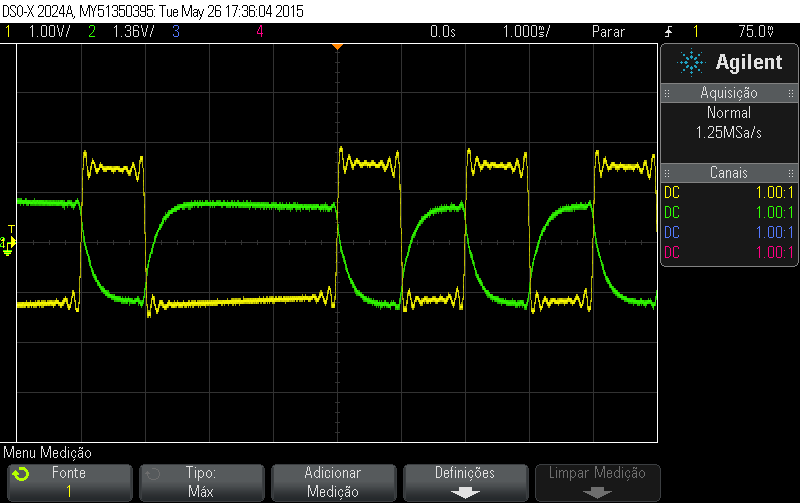
\includegraphics[width=0.5\textwidth]{./dn_y1}~\\
	\caption{sinal de informação, $d_n$,(amarelo) e sinal desmodulado(verde).}
	\label{demod}
\end{figure}

De seguida observa-se como previsto que, uma vez que nos encontramos em sincronismo com o transmissor os sinais resultantes dos detetores de fase, $s_1$ e $s_2$ são a onda de informação com uma componente de alta frequência somada e zero, respetivamente.

\begin{figure}[H]
	\centering
	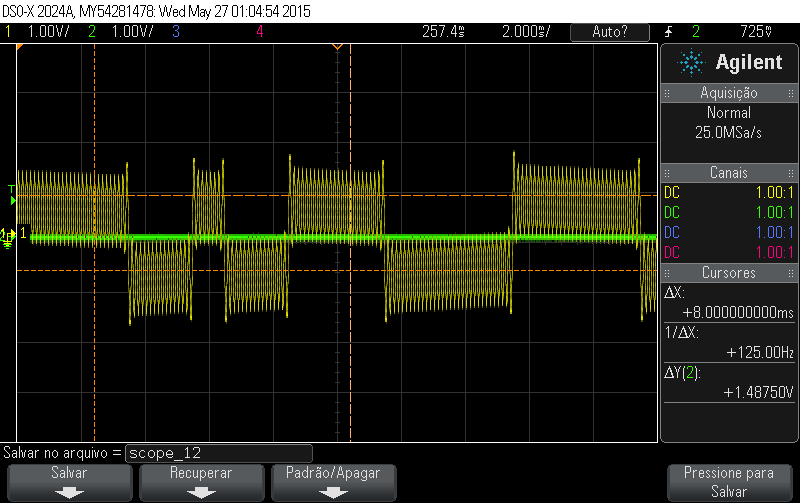
\includegraphics[width=0.5\textwidth]{./s1_s2n}~\\
	\caption{sinal de quadratura, $s_1$,(amarelo) e sinal de fase, $s_2$(verde).}
	\label{s1_s2}
\end{figure}

Agora tem-se uma ilustração do sinal de erro com o sinal desmodulado. O primeiro como previsto, mais uma vez porque o \textit{Costas Loop} está sincronizado, é nulo pois não se tem $\Delta\phi$ e $\Delta f$.

\begin{figure}[H]
	\centering
	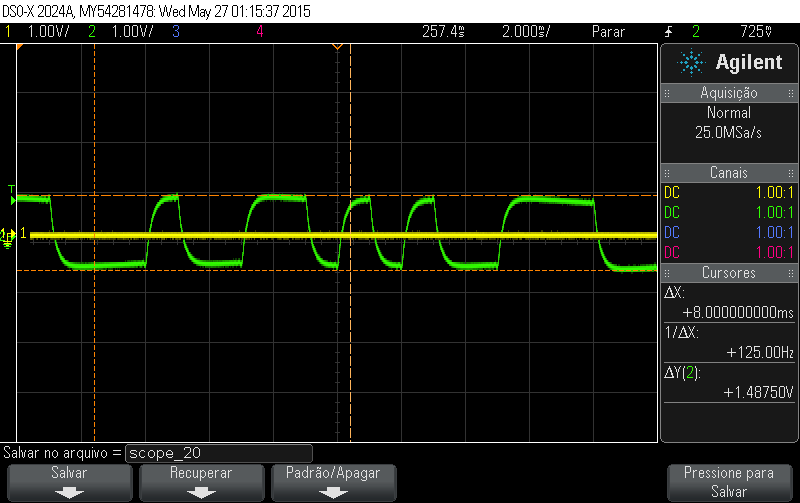
\includegraphics[width=0.5\textwidth]{./erro_y1n}~\\
	\caption{sinal de erro, $\epsilon$,(amarelo) e sinal desmodulado (verde).}
	\label{s1_s2}
\end{figure}

Por fim representa-se os outputs dos data filters e o espetro do sinal desmodulado.

\begin{figure}[H]
	\centering
	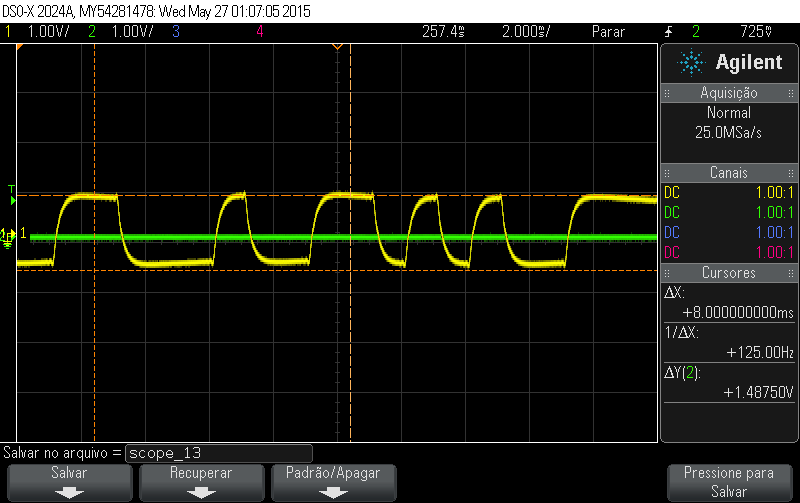
\includegraphics[width=0.5\textwidth]{./y1_y2n}~\\
	\caption{saída do filtro de quadratura(amarelo) e saída do filtro de fase(verde).}
	\label{espetro}
\end{figure}

\begin{figure}[H]
	\centering
	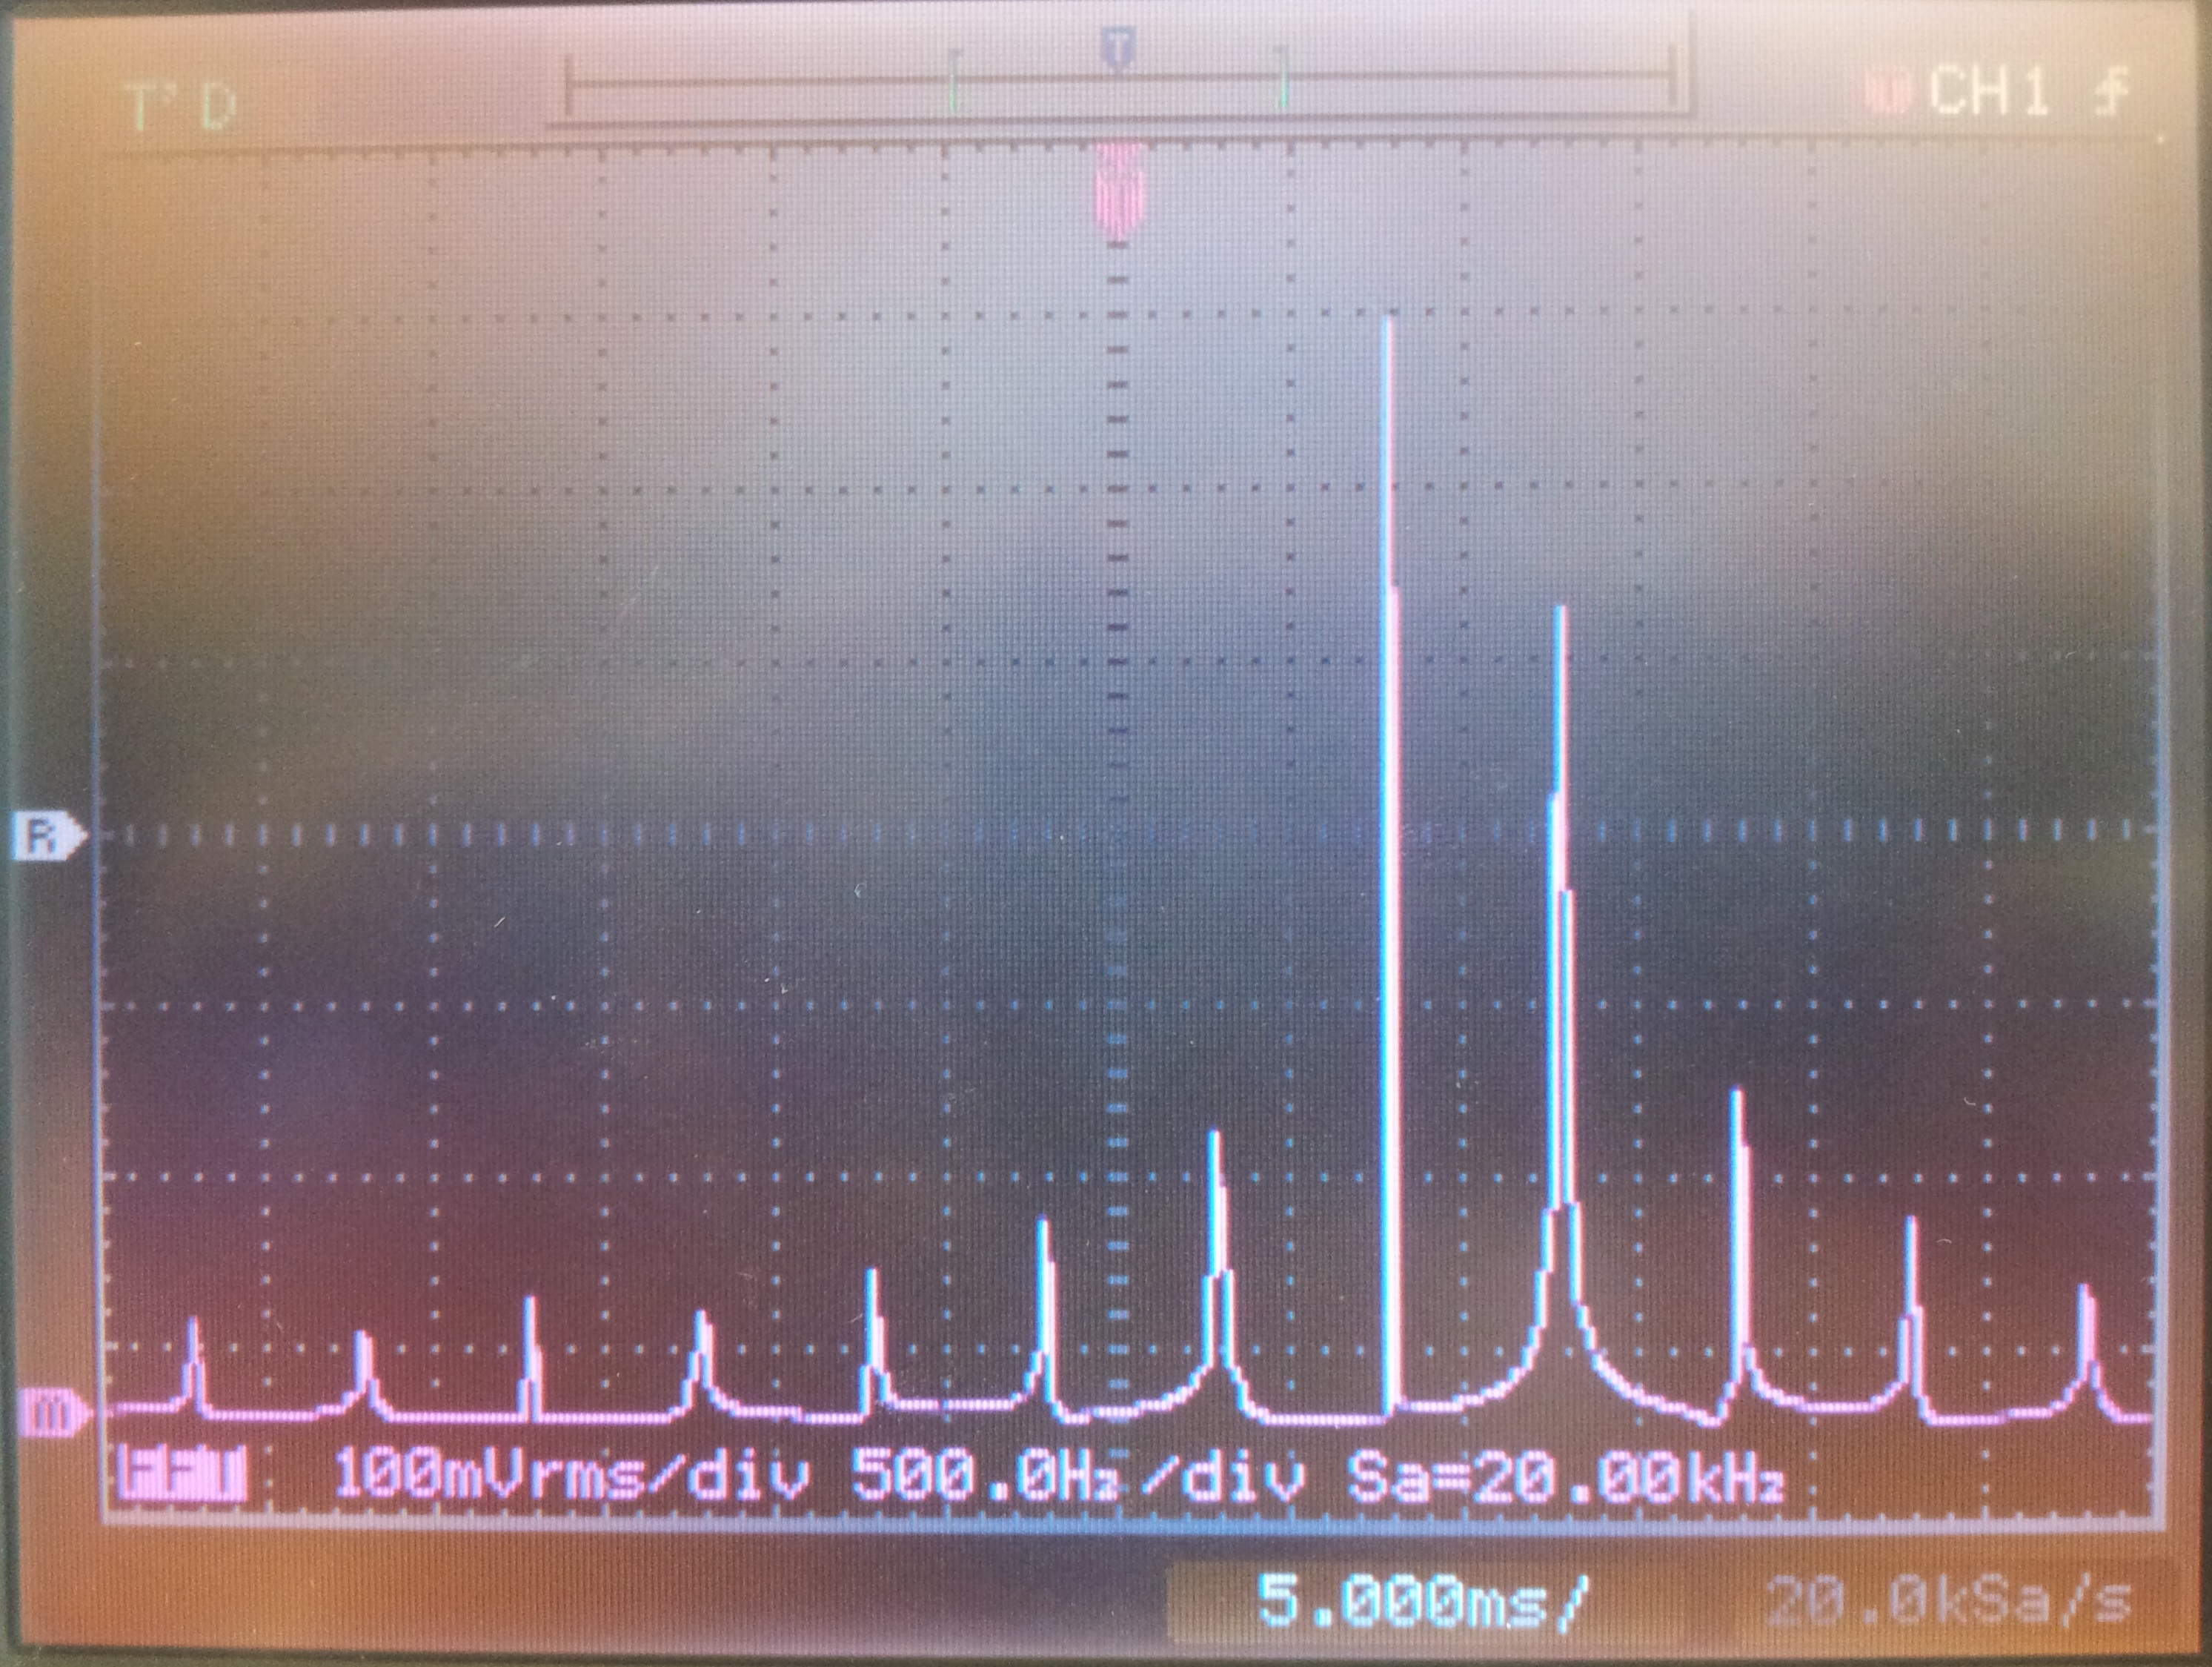
\includegraphics[width=0.5\textwidth]{./espetro}~\\
	\caption{Espetro do sinal desmodulado.}
	\label{espetro}
\end{figure}

Como se pode observar, o espetro trata-se de um $sinc$, com zeros nos múltiplos pares da frequência de $d_n$, $f_d=\frac{f_bit}{2}$, com a escala horizontal com 1kHz/divisão.

\paragraph{8.Transient} \hspace{0pt}

De forma a se poder observar o transitório de aquisição do \textit{Costas Loop}, com a finalidade de poder analisar características adicionais do mesmo, nomeadamente o tempo para se obter sincronismo, fez-se uma análise \textit{transient}. Esta consiste em induzir no circuito um erro de fase elevado, uma vez que é mais simples a alterar a frequência do sinal BPSK, saturando a cada 4000 amostras o valor da variável do erro ( $\epsilon=$ 32767). Observa-se na figura seguinte os sinais de erro e a saìda desmodulada, para um \textit{Loop filter} com frequência de corte, $f_c = 10Hz$:

\begin{figure}[H]
	\centering
	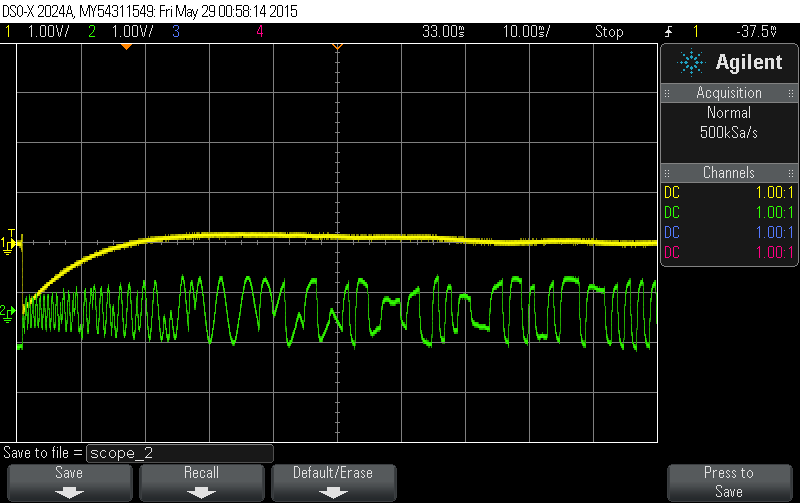
\includegraphics[width=0.5\textwidth]{./transient10Hz}~\\
	\caption{sinal de erro, $\epsilon$, (amarelo) e sinal desmodulado(verde).}
	\label{trans10}
\end{figure}
Observa-se o comportamento esperado do erro com algum overshoot, um curto tempo de estabelecimento e convergindo para 0. Ao mesmo tempo a forma de onda assemelha-se cada vez mais com o sinal de informação. Para este caso tem-se um tempo de sincronismo de $\sim$53ms, tendo em conta a escala horizontal ter 10ms/divisão.

Repetiu-se este teste para um \textit{Loop filter} com frequência de corte, $f_c = 100Hz$, e verificou-se que este circuito sincroniza mais rapidamente com um tempo de sincronismo de $\sim$10ms, tal como se observa na figura seguinte, com a mesma escala horizontal do caso anterior.

\begin{figure}[H]
	\centering
	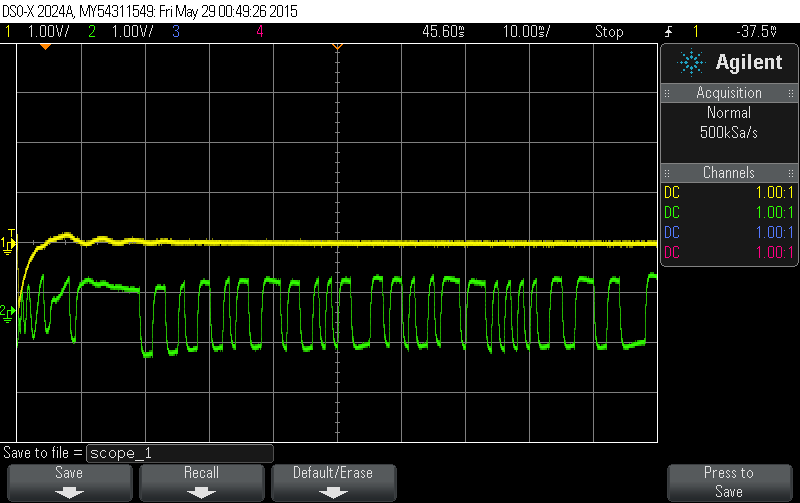
\includegraphics[width=0.5\textwidth]{./transient100Hz}~\\
	\caption{sinal de erro, $\epsilon$, (amarelo) e sinal desmodulado(verde).}
	\label{trans100}
\end{figure}


\section{Conclusão}

\todo{alterar conclusao}

No projeto do oscilador, aprendeu-se como controlar um oscilador a partir de vários parâmetros e o efeito de interpolação linear no mesmo. Como já foi afirmado, a interpolação criou um sinal com maior precisão embora não tenha sido possível observar essa melhoria devido às limitações do equipamento utilizado.

No projeto do transmissor criou-se a primeira parte do modem BPSK, aproveitando o conhecimento adquirido no projeto do oscilador, e observou-se os efeitos da modulação de uma sequência de bits codificada e mapeada, tanto no tempo como na frequência, o que deu para observar pelas inversões de fase presentes no sinal modulado e nas harmónicas do espetro.

\section{Anexos}
\todo{acrescentar codigo da parte 2}
\subsection{Anexo A}
Oscilador Controlado Numericamente:
\lstinputlisting[language=C]{bpsk.c}

\subsection{Anexo B}
Transmissor BPSK:
\lstinputlisting[language=C]{transmissor.c}

\end{document}